\documentclass[twoside]{book}

% Packages required by doxygen
\usepackage{fixltx2e}
\usepackage{calc}
\usepackage{doxygen}
\usepackage[export]{adjustbox} % also loads graphicx
\usepackage{graphicx}
\usepackage[utf8]{inputenc}
\usepackage{makeidx}
\usepackage{multicol}
\usepackage{multirow}
\PassOptionsToPackage{warn}{textcomp}
\usepackage{textcomp}
\usepackage[nointegrals]{wasysym}
\usepackage[table]{xcolor}

% Font selection
\usepackage[T1]{fontenc}
\usepackage[scaled=.90]{helvet}
\usepackage{courier}
\usepackage{amssymb}
\usepackage{sectsty}
\renewcommand{\familydefault}{\sfdefault}
\allsectionsfont{%
  \fontseries{bc}\selectfont%
  \color{darkgray}%
}
\renewcommand{\DoxyLabelFont}{%
  \fontseries{bc}\selectfont%
  \color{darkgray}%
}
\newcommand{\+}{\discretionary{\mbox{\scriptsize$\hookleftarrow$}}{}{}}

% Page & text layout
\usepackage{geometry}
\geometry{%
  a4paper,%
  top=2.5cm,%
  bottom=2.5cm,%
  left=2.5cm,%
  right=2.5cm%
}
\tolerance=750
\hfuzz=15pt
\hbadness=750
\setlength{\emergencystretch}{15pt}
\setlength{\parindent}{0cm}
\setlength{\parskip}{0.2cm}
\makeatletter
\renewcommand{\paragraph}{%
  \@startsection{paragraph}{4}{0ex}{-1.0ex}{1.0ex}{%
    \normalfont\normalsize\bfseries\SS@parafont%
  }%
}
\renewcommand{\subparagraph}{%
  \@startsection{subparagraph}{5}{0ex}{-1.0ex}{1.0ex}{%
    \normalfont\normalsize\bfseries\SS@subparafont%
  }%
}
\makeatother

% Headers & footers
\usepackage{fancyhdr}
\pagestyle{fancyplain}
\fancyhead[LE]{\fancyplain{}{\bfseries\thepage}}
\fancyhead[CE]{\fancyplain{}{}}
\fancyhead[RE]{\fancyplain{}{\bfseries\leftmark}}
\fancyhead[LO]{\fancyplain{}{\bfseries\rightmark}}
\fancyhead[CO]{\fancyplain{}{}}
\fancyhead[RO]{\fancyplain{}{\bfseries\thepage}}
\fancyfoot[LE]{\fancyplain{}{}}
\fancyfoot[CE]{\fancyplain{}{}}
\fancyfoot[RE]{\fancyplain{}{\bfseries\scriptsize Generated on Fri Jun 12 2015 20\+:06\+:51 for L\+O21 by Doxygen }}
\fancyfoot[LO]{\fancyplain{}{\bfseries\scriptsize Generated on Fri Jun 12 2015 20\+:06\+:51 for L\+O21 by Doxygen }}
\fancyfoot[CO]{\fancyplain{}{}}
\fancyfoot[RO]{\fancyplain{}{}}
\renewcommand{\footrulewidth}{0.4pt}
\renewcommand{\chaptermark}[1]{%
  \markboth{#1}{}%
}
\renewcommand{\sectionmark}[1]{%
  \markright{\thesection\ #1}%
}

% Indices & bibliography
\usepackage{natbib}
\usepackage[titles]{tocloft}
\setcounter{tocdepth}{3}
\setcounter{secnumdepth}{5}
\makeindex

% Hyperlinks (required, but should be loaded last)
\usepackage{ifpdf}
\ifpdf
  \usepackage[pdftex,pagebackref=true]{hyperref}
\else
  \usepackage[ps2pdf,pagebackref=true]{hyperref}
\fi
\hypersetup{%
  colorlinks=true,%
  linkcolor=blue,%
  citecolor=blue,%
  unicode%
}

% Custom commands
\newcommand{\clearemptydoublepage}{%
  \newpage{\pagestyle{empty}\cleardoublepage}%
}


%===== C O N T E N T S =====

\begin{document}

% Titlepage & ToC
\hypersetup{pageanchor=false,
             bookmarks=true,
             bookmarksnumbered=true,
             pdfencoding=unicode
            }
\pagenumbering{roman}
\begin{titlepage}
\vspace*{7cm}
\begin{center}%
{\Large L\+O21 \\[1ex]\large 1.\+1 }\\
\vspace*{1cm}
{\large Generated by Doxygen 1.8.9.1}\\
\vspace*{0.5cm}
{\small Fri Jun 12 2015 20:06:51}\\
\end{center}
\end{titlepage}
\clearemptydoublepage
\tableofcontents
\clearemptydoublepage
\pagenumbering{arabic}
\hypersetup{pageanchor=true}

%--- Begin generated contents ---
\chapter{Hierarchical Index}
\section{Class Hierarchy}
This inheritance list is sorted roughly, but not completely, alphabetically\+:\begin{DoxyCompactList}
\item \contentsline{section}{Calendar\+Exception}{\pageref{class_calendar_exception}}{}
\item \contentsline{section}{Choix\+Semaine}{\pageref{class_choix_semaine}}{}
\item \contentsline{section}{Duree}{\pageref{class_duree}}{}
\item \contentsline{section}{Evenement}{\pageref{class_evenement}}{}
\begin{DoxyCompactList}
\item \contentsline{section}{Activite\+Traditionnelle}{\pageref{class_activite_traditionnelle}}{}
\begin{DoxyCompactList}
\item \contentsline{section}{Rdv}{\pageref{class_rdv}}{}
\item \contentsline{section}{Reunion}{\pageref{class_reunion}}{}
\end{DoxyCompactList}
\item \contentsline{section}{Tache}{\pageref{class_tache}}{}
\begin{DoxyCompactList}
\item \contentsline{section}{Tache\+Composite}{\pageref{class_tache_composite}}{}
\item \contentsline{section}{Tache\+Unitaire}{\pageref{class_tache_unitaire}}{}
\begin{DoxyCompactList}
\item \contentsline{section}{Tache\+Unitaire\+Preemptee}{\pageref{class_tache_unitaire_preemptee}}{}
\end{DoxyCompactList}
\end{DoxyCompactList}
\end{DoxyCompactList}
\item \contentsline{section}{Programmation}{\pageref{class_programmation}}{}
\item \contentsline{section}{Programmation\+Manager}{\pageref{class_programmation_manager}}{}
\item \contentsline{section}{Projet}{\pageref{class_projet}}{}
\item \contentsline{section}{Projet\+Manager}{\pageref{class_projet_manager}}{}
\end{DoxyCompactList}

\chapter{Class Index}
\section{Class List}
Here are the classes, structs, unions and interfaces with brief descriptions\+:\begin{DoxyCompactList}
\item\contentsline{section}{\hyperlink{class_activite_traditionnelle}{Activite\+Traditionnelle} \\*Abstrait, herite \hyperlink{class_evenement}{Evenement} toutes les activites autres que les Taches en héritent }{\pageref{class_activite_traditionnelle}}{}
\item\contentsline{section}{\hyperlink{class_calendar_exception}{Calendar\+Exception} \\*Permet la gestion des exceptions dans le programme }{\pageref{class_calendar_exception}}{}
\item\contentsline{section}{\hyperlink{class_choix_semaine}{Choix\+Semaine} \\*Choisir la date a afficher dans l\textquotesingle{}emploi du temps }{\pageref{class_choix_semaine}}{}
\item\contentsline{section}{\hyperlink{class_duree}{Duree} \\*Classe permettant la gestion d\textquotesingle{}une duree }{\pageref{class_duree}}{}
\item\contentsline{section}{\hyperlink{class_evenement}{Evenement} \\*Abstrait toutes les taches et activités programmées en héritent }{\pageref{class_evenement}}{}
\item\contentsline{section}{\hyperlink{class_programmation}{Programmation} \\*Entree de l\textquotesingle{}emploi du temps, referencie un evenement }{\pageref{class_programmation}}{}
\item\contentsline{section}{\hyperlink{class_programmation_manager}{Programmation\+Manager} \\*Regroupe toutes les programmations, l\textquotesingle{}emploi du temps est créé grace a elle }{\pageref{class_programmation_manager}}{}
\item\contentsline{section}{\hyperlink{class_projet}{Projet} \\*Regroupe un ensemble de taches portant sur un certain sujet }{\pageref{class_projet}}{}
\item\contentsline{section}{\hyperlink{class_projet_manager}{Projet\+Manager} \\*Permet la gestion de tous les projets }{\pageref{class_projet_manager}}{}
\item\contentsline{section}{\hyperlink{class_rdv}{Rdv} \\*Sert pour un rendez-\/vous (un seul interlocuteur) }{\pageref{class_rdv}}{}
\item\contentsline{section}{\hyperlink{class_reunion}{Reunion} \\*Classe servant pour les activites avec plusieurss participants }{\pageref{class_reunion}}{}
\item\contentsline{section}{\hyperlink{class_tache}{Tache} \\*Abstrait, herite \hyperlink{class_evenement}{Evenement} toutes les taches en héritent, unité de base d\textquotesingle{}un projet }{\pageref{class_tache}}{}
\item\contentsline{section}{\hyperlink{class_tache_composite}{Tache\+Composite} \\*Regroupement de taches \hyperlink{class_tache}{Tache} complexe, divisée en plusieurs sous Taches, agis comme un projet miniature }{\pageref{class_tache_composite}}{}
\item\contentsline{section}{\hyperlink{class_tache_unitaire}{Tache\+Unitaire} \\*\hyperlink{class_tache}{Tache} simple tache simple, d\textquotesingle{}une certaine durée, a effectuer en une fois }{\pageref{class_tache_unitaire}}{}
\item\contentsline{section}{\hyperlink{class_tache_unitaire_preemptee}{Tache\+Unitaire\+Preemptee} \\*\hyperlink{class_tache}{Tache} Preemptee tache simple, mais faisable en plusieurs fois }{\pageref{class_tache_unitaire_preemptee}}{}
\end{DoxyCompactList}

\chapter{Class Documentation}
\hypertarget{class_activite_traditionnelle}{}\section{Activite\+Traditionnelle Class Reference}
\label{class_activite_traditionnelle}\index{Activite\+Traditionnelle@{Activite\+Traditionnelle}}


Abstrait, herite \hyperlink{class_evenement}{Evenement} toutes les activites autres que les Taches en héritent.  




{\ttfamily \#include $<$evenement.\+h$>$}

Inheritance diagram for Activite\+Traditionnelle\+:\begin{figure}[H]
\begin{center}
\leavevmode
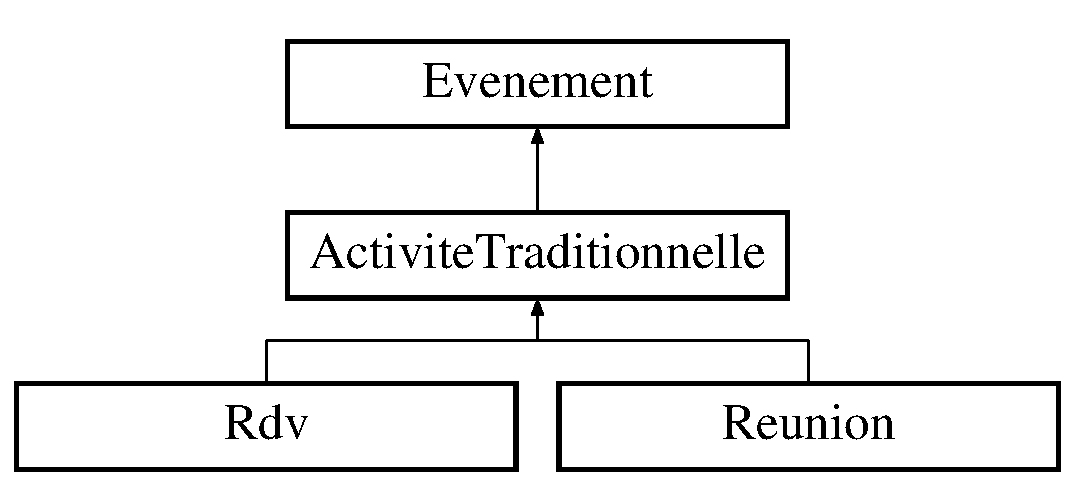
\includegraphics[height=3.000000cm]{class_activite_traditionnelle}
\end{center}
\end{figure}
\subsection*{Public Member Functions}
\begin{DoxyCompactItemize}
\item 
\hypertarget{class_activite_traditionnelle_a8083abcc107dc0a9144176e0ba2ba47c}{}const Q\+String \& {\bfseries get\+Lieu} () const \label{class_activite_traditionnelle_a8083abcc107dc0a9144176e0ba2ba47c}

\item 
\hypertarget{class_activite_traditionnelle_a685b1c01b046576e86a5fe04288176e5}{}virtual \hyperlink{class_duree}{Duree} \hyperlink{class_activite_traditionnelle_a685b1c01b046576e86a5fe04288176e5}{get\+Duree} () const \label{class_activite_traditionnelle_a685b1c01b046576e86a5fe04288176e5}

\begin{DoxyCompactList}\small\item\em renvoit la durée de l\textquotesingle{}evenement la classe evenement ne contient pas d\textquotesingle{}attribut Durée, mais toutes ses sous classes (sauf tache Composite) en possèdent, on décide donc de la créer virtuelle pure \end{DoxyCompactList}\item 
void \hyperlink{class_activite_traditionnelle_a2fb5b53e93f9d191388da7448041553d}{set\+Lieu} (Q\+String nouveau\+Lieu)
\begin{DoxyCompactList}\small\item\em modifie le lieu de l\textquotesingle{}activite \end{DoxyCompactList}\item 
void \hyperlink{class_activite_traditionnelle_ae02975177e5e78ede34eb650d36a73c3}{set\+Duree} (\hyperlink{class_duree}{Duree} nouvelle\+Duree)
\begin{DoxyCompactList}\small\item\em modifie la duree de l\textquotesingle{}activite \end{DoxyCompactList}\end{DoxyCompactItemize}
\subsection*{Protected Member Functions}
\begin{DoxyCompactItemize}
\item 
\hypertarget{class_activite_traditionnelle_a7ef6bdda7b72d06394910f99a00e0ff4}{}{\bfseries Activite\+Traditionnelle} (const Q\+String \&titre, const Q\+String \&lieu, const \hyperlink{class_duree}{Duree} \&duree)\label{class_activite_traditionnelle_a7ef6bdda7b72d06394910f99a00e0ff4}

\end{DoxyCompactItemize}
\subsection*{Private Attributes}
\begin{DoxyCompactItemize}
\item 
\hypertarget{class_activite_traditionnelle_ac5784e2a50475073a1ff7b86798d9a08}{}Q\+String {\bfseries lieu}\label{class_activite_traditionnelle_ac5784e2a50475073a1ff7b86798d9a08}

\item 
\hypertarget{class_activite_traditionnelle_a5cf48113f2174a85db78e9ea7cd32531}{}\hyperlink{class_duree}{Duree} {\bfseries duree}\label{class_activite_traditionnelle_a5cf48113f2174a85db78e9ea7cd32531}

\end{DoxyCompactItemize}
\subsection*{Static Private Attributes}
\begin{DoxyCompactItemize}
\item 
\hypertarget{class_activite_traditionnelle_aa1c0710d6d0e14db65589a0f0b9de29f}{}static int {\bfseries current\+Id} = 0\label{class_activite_traditionnelle_aa1c0710d6d0e14db65589a0f0b9de29f}

\end{DoxyCompactItemize}


\subsection{Detailed Description}
Abstrait, herite \hyperlink{class_evenement}{Evenement} toutes les activites autres que les Taches en héritent. 

\subsection{Member Function Documentation}
\hypertarget{class_activite_traditionnelle_ae02975177e5e78ede34eb650d36a73c3}{}\index{Activite\+Traditionnelle@{Activite\+Traditionnelle}!set\+Duree@{set\+Duree}}
\index{set\+Duree@{set\+Duree}!Activite\+Traditionnelle@{Activite\+Traditionnelle}}
\subsubsection[{set\+Duree}]{\setlength{\rightskip}{0pt plus 5cm}void Activite\+Traditionnelle\+::set\+Duree (
\begin{DoxyParamCaption}
\item[{{\bf Duree}}]{nouvelle\+Duree}
\end{DoxyParamCaption}
)\hspace{0.3cm}{\ttfamily [inline]}}\label{class_activite_traditionnelle_ae02975177e5e78ede34eb650d36a73c3}


modifie la duree de l\textquotesingle{}activite 


\begin{DoxyParams}{Parameters}
{\em nouvelle\+Duree} & \+: nouvlle \hyperlink{class_duree}{Duree} de l\textquotesingle{}activite \\
\hline
\end{DoxyParams}
\hypertarget{class_activite_traditionnelle_a2fb5b53e93f9d191388da7448041553d}{}\index{Activite\+Traditionnelle@{Activite\+Traditionnelle}!set\+Lieu@{set\+Lieu}}
\index{set\+Lieu@{set\+Lieu}!Activite\+Traditionnelle@{Activite\+Traditionnelle}}
\subsubsection[{set\+Lieu}]{\setlength{\rightskip}{0pt plus 5cm}void Activite\+Traditionnelle\+::set\+Lieu (
\begin{DoxyParamCaption}
\item[{Q\+String}]{nouveau\+Lieu}
\end{DoxyParamCaption}
)\hspace{0.3cm}{\ttfamily [inline]}}\label{class_activite_traditionnelle_a2fb5b53e93f9d191388da7448041553d}


modifie le lieu de l\textquotesingle{}activite 


\begin{DoxyParams}{Parameters}
{\em nouveaulieu} & \+: nouveau lieu de l\textquotesingle{}activite \\
\hline
\end{DoxyParams}


The documentation for this class was generated from the following files\+:\begin{DoxyCompactItemize}
\item 
C\+:/\+Users/\+Fixe/\+Desktop/\+Programmation/\+P\+R\+O\+J\+E\+T\+\_\+\+L\+O21/\+Projet/evenement.\+h\item 
C\+:/\+Users/\+Fixe/\+Desktop/\+Programmation/\+P\+R\+O\+J\+E\+T\+\_\+\+L\+O21/\+Projet/evenement.\+cpp\end{DoxyCompactItemize}

\hypertarget{class_calendar_exception}{}\section{Calendar\+Exception Class Reference}
\label{class_calendar_exception}\index{Calendar\+Exception@{Calendar\+Exception}}


permet la gestion des exceptions dans le programme  




{\ttfamily \#include $<$exception.\+h$>$}

\subsection*{Public Member Functions}
\begin{DoxyCompactItemize}
\item 
\hyperlink{class_calendar_exception_afd73d3ab38bc56bb09dfd7674f71d0c3}{Calendar\+Exception} (const Q\+String \&message)
\begin{DoxyCompactList}\small\item\em constructeur \end{DoxyCompactList}\item 
\hypertarget{class_calendar_exception_a5a7ad3b9a770fbc361c809dde840d44c}{}Q\+String {\bfseries get\+Info} () const \label{class_calendar_exception_a5a7ad3b9a770fbc361c809dde840d44c}

\end{DoxyCompactItemize}
\subsection*{Private Attributes}
\begin{DoxyCompactItemize}
\item 
\hypertarget{class_calendar_exception_a0dd66a29c8e82f9cf94da8305576773f}{}Q\+String {\bfseries info}\label{class_calendar_exception_a0dd66a29c8e82f9cf94da8305576773f}

\end{DoxyCompactItemize}


\subsection{Detailed Description}
permet la gestion des exceptions dans le programme 

\subsection{Constructor \& Destructor Documentation}
\hypertarget{class_calendar_exception_afd73d3ab38bc56bb09dfd7674f71d0c3}{}\index{Calendar\+Exception@{Calendar\+Exception}!Calendar\+Exception@{Calendar\+Exception}}
\index{Calendar\+Exception@{Calendar\+Exception}!Calendar\+Exception@{Calendar\+Exception}}
\subsubsection[{Calendar\+Exception}]{\setlength{\rightskip}{0pt plus 5cm}Calendar\+Exception\+::\+Calendar\+Exception (
\begin{DoxyParamCaption}
\item[{const Q\+String \&}]{message}
\end{DoxyParamCaption}
)\hspace{0.3cm}{\ttfamily [inline]}}\label{class_calendar_exception_afd73d3ab38bc56bb09dfd7674f71d0c3}


constructeur 


\begin{DoxyParams}{Parameters}
{\em message} & \+: message a afficher \\
\hline
\end{DoxyParams}


The documentation for this class was generated from the following file\+:\begin{DoxyCompactItemize}
\item 
C\+:/\+Users/\+Fixe/\+Desktop/\+Programmation/\+P\+R\+O\+J\+E\+T\+\_\+\+L\+O21/\+Projet/exception.\+h\end{DoxyCompactItemize}

\hypertarget{class_choix_semaine}{}\section{Choix\+Semaine Class Reference}
\label{class_choix_semaine}\index{Choix\+Semaine@{Choix\+Semaine}}


Choisir la date a afficher dans l\textquotesingle{}emploi du temps.  




{\ttfamily \#include $<$emploidutemps.\+h$>$}



Inherits Q\+Widget.

\subsection*{Public Slots}
\begin{DoxyCompactItemize}
\item 
\hypertarget{class_choix_semaine_aac734d4f6da687961492011f0ead1545}{}void {\bfseries acces\+Ed\+T} ()\label{class_choix_semaine_aac734d4f6da687961492011f0ead1545}

\end{DoxyCompactItemize}
\subsection*{Private Attributes}
\begin{DoxyCompactItemize}
\item 
\hypertarget{class_choix_semaine_a48e322eca1f21a82c0878b4eaea50d7e}{}Q\+Grid\+Layout $\ast$ {\bfseries lay}\label{class_choix_semaine_a48e322eca1f21a82c0878b4eaea50d7e}

\item 
\hypertarget{class_choix_semaine_a739de96c87c9b4dbf4feca009902baf2}{}Q\+Push\+Button $\ast$ {\bfseries valider}\label{class_choix_semaine_a739de96c87c9b4dbf4feca009902baf2}

\item 
\hypertarget{class_choix_semaine_acdf10729c2f640ff1d93910e0cba934f}{}Q\+Label $\ast$ {\bfseries text}\label{class_choix_semaine_acdf10729c2f640ff1d93910e0cba934f}

\item 
\hypertarget{class_choix_semaine_ac925769c0a7319aad3d7f7b8fb77d71f}{}Q\+Date\+Edit $\ast$ {\bfseries choix}\label{class_choix_semaine_ac925769c0a7319aad3d7f7b8fb77d71f}

\end{DoxyCompactItemize}


\subsection{Detailed Description}
Choisir la date a afficher dans l\textquotesingle{}emploi du temps. 

affichage d\textquotesingle{}une semaine permet de creer des programmations ou l\textquotesingle{}export de l\textquotesingle{}emploi du temps 

The documentation for this class was generated from the following files\+:\begin{DoxyCompactItemize}
\item 
C\+:/\+Users/\+Fixe/\+Desktop/\+Programmation/\+P\+R\+O\+J\+E\+T\+\_\+\+L\+O21/\+Projet/emploidutemps.\+h\item 
C\+:/\+Users/\+Fixe/\+Desktop/\+Programmation/\+P\+R\+O\+J\+E\+T\+\_\+\+L\+O21/\+Projet/emploidutemps.\+cpp\end{DoxyCompactItemize}

\hypertarget{class_duree}{}\section{Duree Class Reference}
\label{class_duree}\index{Duree@{Duree}}


Classe permettant la gestion d\textquotesingle{}une duree.  




{\ttfamily \#include $<$duree.\+h$>$}

\subsection*{Public Member Functions}
\begin{DoxyCompactItemize}
\item 
\hyperlink{class_duree_a9031ee4cb937a2cb48a833924e0d8175}{Duree} (unsigned int h, unsigned int m)
\begin{DoxyCompactList}\small\item\em Constructeur deux arguments \+: heure et minutes. \end{DoxyCompactList}\item 
\hyperlink{class_duree_a29ce444d85f2870058025ce5db0802a5}{Duree} (unsigned int m=0)
\begin{DoxyCompactList}\small\item\em surcharge Constructeur unargument \+: minutes \end{DoxyCompactList}\item 
\hyperlink{class_duree_a419162e60eca1314a3611752ab3d68cd}{Duree} (const \hyperlink{class_duree}{Duree} \&other)
\begin{DoxyCompactList}\small\item\em Constructeur de recopie. \end{DoxyCompactList}\item 
void \hyperlink{class_duree_a9d38c17651a31e52a19252a891933da4}{set\+Duree} (unsigned int heures, unsigned int minutes)
\begin{DoxyCompactList}\small\item\em modifier la duree \end{DoxyCompactList}\item 
void \hyperlink{class_duree_acf2e742070a8b558ff7c5fab3f2ec472}{set\+Duree} (unsigned int minutes)
\begin{DoxyCompactList}\small\item\em surcharge pour modifier heure \end{DoxyCompactList}\item 
\hypertarget{class_duree_a0e25c3388ea08f41140aee71ffaae4ee}{}unsigned int {\bfseries get\+Duree\+En\+Minutes} () const \label{class_duree_a0e25c3388ea08f41140aee71ffaae4ee}

\item 
\hypertarget{class_duree_acaf629d6df6668a2c2d9a7f5bffeb9e1}{}double {\bfseries get\+Duree\+En\+Heures} () const \label{class_duree_acaf629d6df6668a2c2d9a7f5bffeb9e1}

\item 
\hypertarget{class_duree_a3a6bfde3c641f15c68ac4f88303ce275}{}int {\bfseries get\+Reste\+Duree\+En\+Minutes} () const \label{class_duree_a3a6bfde3c641f15c68ac4f88303ce275}

\item 
\hypertarget{class_duree_aa44bd9ae4f27fe00204543feeaefe2ca}{}\hyperlink{class_duree}{Duree} {\bfseries operator+} (unsigned int min) const \label{class_duree_aa44bd9ae4f27fe00204543feeaefe2ca}

\item 
\hypertarget{class_duree_adf484fa269dc25a6247cd25795bd72ea}{}\hyperlink{class_duree}{Duree} {\bfseries operator-\/} (\hyperlink{class_duree}{Duree} const \&other) const \label{class_duree_adf484fa269dc25a6247cd25795bd72ea}

\item 
\hypertarget{class_duree_a9866be4c92f15c2c5ddd0ccdaab566df}{}\hyperlink{class_duree}{Duree} {\bfseries operator+=} (\hyperlink{class_duree}{Duree} const \&other)\label{class_duree_a9866be4c92f15c2c5ddd0ccdaab566df}

\item 
\hypertarget{class_duree_a243ef035ea34f4c6e34f928b8e9924ab}{}\hyperlink{class_duree}{Duree} {\bfseries operator-\/=} (\hyperlink{class_duree}{Duree} const \&other)\label{class_duree_a243ef035ea34f4c6e34f928b8e9924ab}

\item 
\hypertarget{class_duree_a230a64859fa89a4d3c983d96af0a5925}{}bool {\bfseries operator==} (\hyperlink{class_duree}{Duree} const \&other) const \label{class_duree_a230a64859fa89a4d3c983d96af0a5925}

\item 
\hypertarget{class_duree_a91e334a82cec62fd43e4c80db0acfe13}{}bool {\bfseries operator$>$=} (\hyperlink{class_duree}{Duree} const \&other) const \label{class_duree_a91e334a82cec62fd43e4c80db0acfe13}

\item 
\hypertarget{class_duree_ae82a6ed05f23dde893b83b5f31dd20a2}{}bool {\bfseries operator$<$=} (\hyperlink{class_duree}{Duree} const \&other) const \label{class_duree_ae82a6ed05f23dde893b83b5f31dd20a2}

\item 
\hypertarget{class_duree_a2dc45a74a26a1fd35605aca6b321208b}{}bool {\bfseries operator$<$} (\hyperlink{class_duree}{Duree} const \&other) const \label{class_duree_a2dc45a74a26a1fd35605aca6b321208b}

\item 
\hypertarget{class_duree_ad76fa253fe864da9713fefc77f12e181}{}bool {\bfseries operator$>$} (\hyperlink{class_duree}{Duree} const \&other) const \label{class_duree_ad76fa253fe864da9713fefc77f12e181}

\end{DoxyCompactItemize}
\subsection*{Private Attributes}
\begin{DoxyCompactItemize}
\item 
unsigned int \hyperlink{class_duree_a27de9771cfe31979ebed0b01eeb946cf}{nb\+Minutes}
\end{DoxyCompactItemize}


\subsection{Detailed Description}
Classe permettant la gestion d\textquotesingle{}une duree. 

La classe gere la lecture d\textquotesingle{}une liste de morceaux 

\subsection{Constructor \& Destructor Documentation}
\hypertarget{class_duree_a9031ee4cb937a2cb48a833924e0d8175}{}\index{Duree@{Duree}!Duree@{Duree}}
\index{Duree@{Duree}!Duree@{Duree}}
\subsubsection[{Duree}]{\setlength{\rightskip}{0pt plus 5cm}Duree\+::\+Duree (
\begin{DoxyParamCaption}
\item[{unsigned int}]{h, }
\item[{unsigned int}]{m}
\end{DoxyParamCaption}
)\hspace{0.3cm}{\ttfamily [inline]}}\label{class_duree_a9031ee4cb937a2cb48a833924e0d8175}


Constructeur deux arguments \+: heure et minutes. 


\begin{DoxyParams}{Parameters}
{\em h} & nombre d\textquotesingle{}heures \\
\hline
{\em m} & nombre de minutes (fonctionne si m$>$60) \\
\hline
\end{DoxyParams}
\hypertarget{class_duree_a29ce444d85f2870058025ce5db0802a5}{}\index{Duree@{Duree}!Duree@{Duree}}
\index{Duree@{Duree}!Duree@{Duree}}
\subsubsection[{Duree}]{\setlength{\rightskip}{0pt plus 5cm}Duree\+::\+Duree (
\begin{DoxyParamCaption}
\item[{unsigned int}]{m = {\ttfamily 0}}
\end{DoxyParamCaption}
)\hspace{0.3cm}{\ttfamily [inline]}}\label{class_duree_a29ce444d85f2870058025ce5db0802a5}


surcharge Constructeur unargument \+: minutes 


\begin{DoxyParams}{Parameters}
{\em m} & nombre de minutes (fonctionne si m$>$60) \\
\hline
\end{DoxyParams}
\hypertarget{class_duree_a419162e60eca1314a3611752ab3d68cd}{}\index{Duree@{Duree}!Duree@{Duree}}
\index{Duree@{Duree}!Duree@{Duree}}
\subsubsection[{Duree}]{\setlength{\rightskip}{0pt plus 5cm}Duree\+::\+Duree (
\begin{DoxyParamCaption}
\item[{const {\bf Duree} \&}]{other}
\end{DoxyParamCaption}
)\hspace{0.3cm}{\ttfamily [inline]}}\label{class_duree_a419162e60eca1314a3611752ab3d68cd}


Constructeur de recopie. 


\begin{DoxyParams}{Parameters}
{\em other} & \hyperlink{class_duree}{Duree} a recopier \\
\hline
\end{DoxyParams}


\subsection{Member Function Documentation}
\hypertarget{class_duree_a9d38c17651a31e52a19252a891933da4}{}\index{Duree@{Duree}!set\+Duree@{set\+Duree}}
\index{set\+Duree@{set\+Duree}!Duree@{Duree}}
\subsubsection[{set\+Duree}]{\setlength{\rightskip}{0pt plus 5cm}void Duree\+::set\+Duree (
\begin{DoxyParamCaption}
\item[{unsigned int}]{heures, }
\item[{unsigned int}]{minutes}
\end{DoxyParamCaption}
)\hspace{0.3cm}{\ttfamily [inline]}}\label{class_duree_a9d38c17651a31e52a19252a891933da4}


modifier la duree 


\begin{DoxyParams}{Parameters}
{\em heures} & nombre d\textquotesingle{}heures \\
\hline
{\em minutes} & nombre de minute (fonctionne si minutes$>$60) \\
\hline
\end{DoxyParams}
\hypertarget{class_duree_acf2e742070a8b558ff7c5fab3f2ec472}{}\index{Duree@{Duree}!set\+Duree@{set\+Duree}}
\index{set\+Duree@{set\+Duree}!Duree@{Duree}}
\subsubsection[{set\+Duree}]{\setlength{\rightskip}{0pt plus 5cm}void Duree\+::set\+Duree (
\begin{DoxyParamCaption}
\item[{unsigned int}]{minutes}
\end{DoxyParamCaption}
)\hspace{0.3cm}{\ttfamily [inline]}}\label{class_duree_acf2e742070a8b558ff7c5fab3f2ec472}


surcharge pour modifier heure 


\begin{DoxyParams}{Parameters}
{\em minutes} & duree totale en minute \\
\hline
\end{DoxyParams}


\subsection{Member Data Documentation}
\hypertarget{class_duree_a27de9771cfe31979ebed0b01eeb946cf}{}\index{Duree@{Duree}!nb\+Minutes@{nb\+Minutes}}
\index{nb\+Minutes@{nb\+Minutes}!Duree@{Duree}}
\subsubsection[{nb\+Minutes}]{\setlength{\rightskip}{0pt plus 5cm}unsigned int Duree\+::nb\+Minutes\hspace{0.3cm}{\ttfamily [private]}}\label{class_duree_a27de9771cfe31979ebed0b01eeb946cf}
\hyperlink{class_duree}{Duree} en minute 

The documentation for this class was generated from the following files\+:\begin{DoxyCompactItemize}
\item 
C\+:/\+Users/\+Fixe/\+Desktop/\+Programmation/\+P\+R\+O\+J\+E\+T\+\_\+\+L\+O21/\+Projet/duree.\+h\item 
C\+:/\+Users/\+Fixe/\+Desktop/\+Programmation/\+P\+R\+O\+J\+E\+T\+\_\+\+L\+O21/\+Projet/duree.\+cpp\end{DoxyCompactItemize}

\hypertarget{class_evenement}{}\section{Evenement Class Reference}
\label{class_evenement}\index{Evenement@{Evenement}}


Abstrait toutes les taches et activités programmées en héritent.  




{\ttfamily \#include $<$evenement.\+h$>$}

Inheritance diagram for Evenement\+:\begin{figure}[H]
\begin{center}
\leavevmode
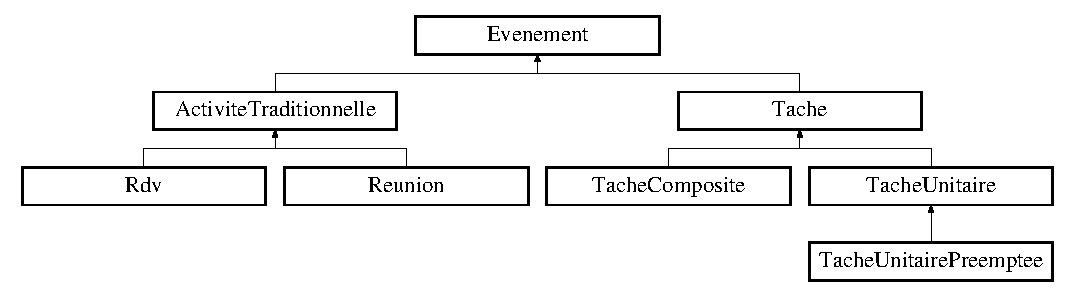
\includegraphics[height=3.544304cm]{class_evenement}
\end{center}
\end{figure}
\subsection*{Public Member Functions}
\begin{DoxyCompactItemize}
\item 
\hypertarget{class_evenement_a28a67eded4a392879afc44c6a37a6c94}{}int {\bfseries get\+Id} () const \label{class_evenement_a28a67eded4a392879afc44c6a37a6c94}

\item 
\hypertarget{class_evenement_adf40be537c30e34f70cd0e62c0239607}{}const Q\+String \& {\bfseries get\+Titre} () const \label{class_evenement_adf40be537c30e34f70cd0e62c0239607}

\item 
void \hyperlink{class_evenement_ac74631f811449f10b2069f5d0a2f2ad2}{set\+Titre} (const Q\+String \&t)
\begin{DoxyCompactList}\small\item\em permet de modifier le titre de l\textquotesingle{}event \end{DoxyCompactList}\item 
\hypertarget{class_evenement_ae19e4e2d2c5ee5a78d7eb99f3ddecf3a}{}virtual \hyperlink{class_duree}{Duree} \hyperlink{class_evenement_ae19e4e2d2c5ee5a78d7eb99f3ddecf3a}{get\+Duree} () const =0\label{class_evenement_ae19e4e2d2c5ee5a78d7eb99f3ddecf3a}

\begin{DoxyCompactList}\small\item\em renvoit la durée de l\textquotesingle{}evenement la classe evenement ne contient pas d\textquotesingle{}attribut Durée, mais toutes ses sous classes (sauf tache Composite) en possèdent, on décide donc de la créer virtuelle pure \end{DoxyCompactList}\item 
virtual void \hyperlink{class_evenement_ad4baf55b2e276b86ca5c5fd77c01f5d3}{set\+Programme} (bool effectue)
\begin{DoxyCompactList}\small\item\em change l\textquotesingle{}etat (programme/non programme) \end{DoxyCompactList}\item 
\hypertarget{class_evenement_af8af8009f07901c4017636c310082e66}{}bool {\bfseries is\+Programme} ()\label{class_evenement_af8af8009f07901c4017636c310082e66}

\end{DoxyCompactItemize}
\subsection*{Protected Member Functions}
\begin{DoxyCompactItemize}
\item 
\hypertarget{class_evenement_aeba272d8dceb6584f479232f68cf589b}{}{\bfseries Evenement} (int id, const Q\+String \&t)\label{class_evenement_aeba272d8dceb6584f479232f68cf589b}

\end{DoxyCompactItemize}
\subsection*{Private Attributes}
\begin{DoxyCompactItemize}
\item 
\hypertarget{class_evenement_a5e3e95ca2853b020205a607d3f8d254b}{}Q\+String {\bfseries titre}\label{class_evenement_a5e3e95ca2853b020205a607d3f8d254b}

\item 
\hypertarget{class_evenement_a3f90a64a77837a821463422608603b88}{}int {\bfseries id}\label{class_evenement_a3f90a64a77837a821463422608603b88}

\item 
\hypertarget{class_evenement_a9ebea5ef4d9e3a92619d2da9e97b7b4b}{}bool {\bfseries prog}\label{class_evenement_a9ebea5ef4d9e3a92619d2da9e97b7b4b}

\end{DoxyCompactItemize}


\subsection{Detailed Description}
Abstrait toutes les taches et activités programmées en héritent. 

\subsection{Member Function Documentation}
\hypertarget{class_evenement_ad4baf55b2e276b86ca5c5fd77c01f5d3}{}\index{Evenement@{Evenement}!set\+Programme@{set\+Programme}}
\index{set\+Programme@{set\+Programme}!Evenement@{Evenement}}
\subsubsection[{set\+Programme}]{\setlength{\rightskip}{0pt plus 5cm}virtual void Evenement\+::set\+Programme (
\begin{DoxyParamCaption}
\item[{bool}]{effectue}
\end{DoxyParamCaption}
)\hspace{0.3cm}{\ttfamily [inline]}, {\ttfamily [virtual]}}\label{class_evenement_ad4baf55b2e276b86ca5c5fd77c01f5d3}


change l\textquotesingle{}etat (programme/non programme) 


\begin{DoxyParams}{Parameters}
{\em effectue} & \+: dis si l\textquotesingle{}activite est programmée ou non \\
\hline
\end{DoxyParams}


Reimplemented in \hyperlink{class_tache_a662db9ee24100a3d52853542c98dadf7}{Tache}.

\hypertarget{class_evenement_ac74631f811449f10b2069f5d0a2f2ad2}{}\index{Evenement@{Evenement}!set\+Titre@{set\+Titre}}
\index{set\+Titre@{set\+Titre}!Evenement@{Evenement}}
\subsubsection[{set\+Titre}]{\setlength{\rightskip}{0pt plus 5cm}void Evenement\+::set\+Titre (
\begin{DoxyParamCaption}
\item[{const Q\+String \&}]{t}
\end{DoxyParamCaption}
)}\label{class_evenement_ac74631f811449f10b2069f5d0a2f2ad2}


permet de modifier le titre de l\textquotesingle{}event 


\begin{DoxyParams}{Parameters}
{\em t} & nouveau titre \\
\hline
\end{DoxyParams}


The documentation for this class was generated from the following files\+:\begin{DoxyCompactItemize}
\item 
C\+:/\+Users/\+Fixe/\+Desktop/\+Programmation/\+P\+R\+O\+J\+E\+T\+\_\+\+L\+O21/\+Projet/evenement.\+h\item 
C\+:/\+Users/\+Fixe/\+Desktop/\+Programmation/\+P\+R\+O\+J\+E\+T\+\_\+\+L\+O21/\+Projet/evenement.\+cpp\end{DoxyCompactItemize}

\hypertarget{class_programmation}{}\section{Programmation Class Reference}
\label{class_programmation}\index{Programmation@{Programmation}}


entree de l\textquotesingle{}emploi du temps, referencie un evenement  




{\ttfamily \#include $<$programmation.\+h$>$}

\subsection*{Public Member Functions}
\begin{DoxyCompactItemize}
\item 
\hypertarget{class_programmation_ad55acbdd7059371d5b2ebf0a2b43597a}{}const Q\+Date \& {\bfseries get\+Date\+Choisie} () const \label{class_programmation_ad55acbdd7059371d5b2ebf0a2b43597a}

\item 
\hypertarget{class_programmation_a95a28145c5eca80db8e7804404519595}{}const Q\+Time \& {\bfseries get\+Horaire\+Choisi} () const \label{class_programmation_a95a28145c5eca80db8e7804404519595}

\item 
\hypertarget{class_programmation_a0cbf62a3f0efd174de69e7019e0dc8ed}{}const \hyperlink{class_duree}{Duree} \& {\bfseries get\+Duree} () const \label{class_programmation_a0cbf62a3f0efd174de69e7019e0dc8ed}

\item 
\hypertarget{class_programmation_a7cd81da6d10a29782d21e6eb0d0910d6}{}void {\bfseries set\+Date\+Choisie} (Q\+Date d)\label{class_programmation_a7cd81da6d10a29782d21e6eb0d0910d6}

\item 
\hypertarget{class_programmation_ab8d0445e7fcca977527e6cdcc6237fba}{}void {\bfseries set\+Horaire\+Choisi} (Q\+Time t)\label{class_programmation_ab8d0445e7fcca977527e6cdcc6237fba}

\item 
\hypertarget{class_programmation_a54812c3cd58224600a3d62738946a3c4}{}void {\bfseries set\+Duree} (\hyperlink{class_duree}{Duree} d)\label{class_programmation_a54812c3cd58224600a3d62738946a3c4}

\item 
\hypertarget{class_programmation_ab4373ed1d42d39a830fdbac7385e69eb}{}int {\bfseries get\+Id} () const \label{class_programmation_ab4373ed1d42d39a830fdbac7385e69eb}

\item 
\hypertarget{class_programmation_afdb51dc8924974a73bc750096ae0151c}{}\hyperlink{class_evenement}{Evenement} $\ast$ {\bfseries get\+Event} ()\label{class_programmation_afdb51dc8924974a73bc750096ae0151c}

\item 
\hypertarget{class_programmation_a8a8e262d61a00c2e2d46c1aad7c895ff}{}const Q\+Time {\bfseries get\+Horaire\+Fin} () const \label{class_programmation_a8a8e262d61a00c2e2d46c1aad7c895ff}

\item 
\hypertarget{class_programmation_ae5e3c4dc5b6310e1b054a64b3eaee5fe}{}bool {\bfseries operator$>$} (const \hyperlink{class_programmation}{Programmation} \&other) const \label{class_programmation_ae5e3c4dc5b6310e1b054a64b3eaee5fe}

\item 
\hypertarget{class_programmation_a47bd954f67af45e8543efe792be05395}{}bool {\bfseries operator$<$} (const \hyperlink{class_programmation}{Programmation} \&other) const \label{class_programmation_a47bd954f67af45e8543efe792be05395}

\end{DoxyCompactItemize}
\subsection*{Private Member Functions}
\begin{DoxyCompactItemize}
\item 
\hypertarget{class_programmation_a7a32bea3ba1f02444f74dd38baaf9e8d}{}{\bfseries Programmation} (\hyperlink{class_evenement}{Evenement} $\ast$event, const Q\+Date \&date\+Choisie, const Q\+Time \&horaire\+Choisi, \hyperlink{class_duree}{Duree} dur=\hyperlink{class_duree}{Duree}(0))\label{class_programmation_a7a32bea3ba1f02444f74dd38baaf9e8d}

\item 
\hypertarget{class_programmation_ac999e116031fbc745dc32e0e6f8e2732}{}\hyperlink{class_programmation}{Programmation} {\bfseries operator=} (\hyperlink{class_programmation}{Programmation} \&other)\label{class_programmation_ac999e116031fbc745dc32e0e6f8e2732}

\item 
\hypertarget{class_programmation_ad6600e4dcea95c4f91e211b3a1700bce}{}{\bfseries Programmation} (\hyperlink{class_programmation}{Programmation} \&other)\label{class_programmation_ad6600e4dcea95c4f91e211b3a1700bce}

\end{DoxyCompactItemize}
\subsection*{Private Attributes}
\begin{DoxyCompactItemize}
\item 
\hypertarget{class_programmation_a94015d566f0afca80fea7b888f93c727}{}int {\bfseries id}\label{class_programmation_a94015d566f0afca80fea7b888f93c727}

\item 
\hypertarget{class_programmation_ac4d9c0b80ab3b203122b94d690871100}{}Q\+Date {\bfseries date\+Choisie}\label{class_programmation_ac4d9c0b80ab3b203122b94d690871100}

\item 
\hypertarget{class_programmation_a7b51bcd99f633bb34903c9471ccc792b}{}Q\+Time {\bfseries horaire\+Choisi}\label{class_programmation_a7b51bcd99f633bb34903c9471ccc792b}

\item 
\hypertarget{class_programmation_a1cdf70965e5af5a917e3bc7c922a735e}{}\hyperlink{class_duree}{Duree} {\bfseries duree}\label{class_programmation_a1cdf70965e5af5a917e3bc7c922a735e}

\item 
\hypertarget{class_programmation_ac64a1d3793894549ff5b3a2c9015aef2}{}\hyperlink{class_evenement}{Evenement} $\ast$ {\bfseries evt}\label{class_programmation_ac64a1d3793894549ff5b3a2c9015aef2}

\end{DoxyCompactItemize}
\subsection*{Static Private Attributes}
\begin{DoxyCompactItemize}
\item 
\hypertarget{class_programmation_a7a72d00fe285adc58d40405cb7b709d5}{}static int {\bfseries current\+Id} = 0\label{class_programmation_a7a72d00fe285adc58d40405cb7b709d5}

\end{DoxyCompactItemize}
\subsection*{Friends}
\begin{DoxyCompactItemize}
\item 
\hypertarget{class_programmation_ade7bfcbf8cec66b12064c8ff25993d73}{}class {\bfseries Programmation\+Manager}\label{class_programmation_ade7bfcbf8cec66b12064c8ff25993d73}

\end{DoxyCompactItemize}


\subsection{Detailed Description}
entree de l\textquotesingle{}emploi du temps, referencie un evenement 

The documentation for this class was generated from the following files\+:\begin{DoxyCompactItemize}
\item 
C\+:/\+Users/\+Fixe/\+Desktop/\+Programmation/\+P\+R\+O\+J\+E\+T\+\_\+\+L\+O21/\+Projet/programmation.\+h\item 
C\+:/\+Users/\+Fixe/\+Desktop/\+Programmation/\+P\+R\+O\+J\+E\+T\+\_\+\+L\+O21/\+Projet/programmation.\+cpp\end{DoxyCompactItemize}

\hypertarget{class_programmation_manager}{}\section{Programmation\+Manager Class Reference}
\label{class_programmation_manager}\index{Programmation\+Manager@{Programmation\+Manager}}


regroupe toutes les programmations, l\textquotesingle{}emploi du temps est créé grace a elle  




{\ttfamily \#include $<$programmation.\+h$>$}

\subsection*{Public Member Functions}
\begin{DoxyCompactItemize}
\item 
\hypertarget{class_programmation_manager_a975a9226a49d850f54d5f64a407969b2}{}bool {\bfseries creneaulibre} (const Q\+Date \&da, const Q\+Time \&h, const \hyperlink{class_duree}{Duree} \&du)\label{class_programmation_manager_a975a9226a49d850f54d5f64a407969b2}

\item 
void \hyperlink{class_programmation_manager_ad2152e1d6f91acc5542caf33252640d0}{creer\+Programmation} (\hyperlink{class_evenement}{Evenement} $\ast$event, Q\+Date date\+Choisie, Q\+Time horaire\+Choisi)
\begin{DoxyCompactList}\small\item\em crée une programmation pour un evenement choisi \end{DoxyCompactList}\item 
\hyperlink{class_programmation}{Programmation} \& \hyperlink{class_programmation_manager_a7b7a03494972c8140d520f3bc24abe0a}{get\+Programmation} (int id)
\begin{DoxyCompactList}\small\item\em cherche une programmation \end{DoxyCompactList}\item 
\hyperlink{class_programmation}{Programmation} \& \hyperlink{class_programmation_manager_a012b8871019408b1a0bc4bb40696fa08}{get\+Derniere\+Programmation} (\hyperlink{class_evenement}{Evenement} $\ast$evt)
\begin{DoxyCompactList}\small\item\em cherche une programmation relative a un evenement \end{DoxyCompactList}\item 
\hypertarget{class_programmation_manager_a135184cab7050ec7568eab43f46abd02}{}const std\+::vector$<$ \hyperlink{class_programmation}{Programmation} $\ast$ $>$ \& {\bfseries get\+Programmations} () const \label{class_programmation_manager_a135184cab7050ec7568eab43f46abd02}

\item 
\hypertarget{class_programmation_manager_a3305db243c119907a10646d504c99484}{}std\+::vector$<$ \hyperlink{class_programmation}{Programmation} $\ast$ $>$ {\bfseries get\+Semaine} (Q\+Date \&date) const \label{class_programmation_manager_a3305db243c119907a10646d504c99484}

\item 
void \hyperlink{class_programmation_manager_af1a24f310ba7b622d4e2641af7c069cf}{supprimer\+Programmations\+Evt} (const Q\+String p)
\begin{DoxyCompactList}\small\item\em supprime les programmations en rapport a un evenement \end{DoxyCompactList}\item 
void \hyperlink{class_programmation_manager_aa0dea8a1860f1fca3a462ea77ca1dc09}{supprimer\+Programmation} (int id)
\begin{DoxyCompactList}\small\item\em supprime la programmation d\textquotesingle{}id id \end{DoxyCompactList}\end{DoxyCompactItemize}
\subsection*{Static Public Member Functions}
\begin{DoxyCompactItemize}
\item 
\hypertarget{class_programmation_manager_a9da2fc647972756d1f8cdf91d4017c25}{}static \hyperlink{class_programmation_manager}{Programmation\+Manager} \& {\bfseries get\+Instance} ()\label{class_programmation_manager_a9da2fc647972756d1f8cdf91d4017c25}

\item 
\hypertarget{class_programmation_manager_a94e3fcb28ea7c632dc6750c33949d712}{}static void {\bfseries liberer\+Instance} ()\label{class_programmation_manager_a94e3fcb28ea7c632dc6750c33949d712}

\end{DoxyCompactItemize}
\subsection*{Private Member Functions}
\begin{DoxyCompactItemize}
\item 
\hyperlink{class_programmation}{Programmation} $\ast$ \hyperlink{class_programmation_manager_a7bb1d14ed92cf719d2eb8952b5c59dd9}{trouver\+Programmation} (int id) const 
\begin{DoxyCompactList}\small\item\em cherche une programmation \end{DoxyCompactList}\item 
\hyperlink{class_programmation}{Programmation} $\ast$ \hyperlink{class_programmation_manager_a39d428d422191a382fa4365e0f3e4b04}{trouver\+Derniere\+Programmation} (\hyperlink{class_evenement}{Evenement} $\ast$evt) const 
\begin{DoxyCompactList}\small\item\em cherche une programmation relative a un evenement \end{DoxyCompactList}\item 
\hyperlink{class_programmation}{Programmation} $\ast$ \hyperlink{class_programmation_manager_a8f25dc83efdf00ab879df4f73fdad51f}{create\+Prog\+Preemptee} (\hyperlink{class_evenement}{Evenement} $\ast$event, Q\+Date date, Q\+Time horaire)
\begin{DoxyCompactList}\small\item\em sert pour les tache preemptee fera apparaitre une fenetre pour choisir la duree de la programmation \end{DoxyCompactList}\item 
void \hyperlink{class_programmation_manager_a3e84c7978bdce13ddcaef7e706ac2d49}{add\+Item} (\hyperlink{class_programmation}{Programmation} $\ast$t)
\begin{DoxyCompactList}\small\item\em ajoute une programmation a la liste globale \end{DoxyCompactList}\end{DoxyCompactItemize}
\subsection*{Private Attributes}
\begin{DoxyCompactItemize}
\item 
\hypertarget{class_programmation_manager_a2c28e7737241fc6612daccaca5b512e8}{}std\+::vector$<$ \hyperlink{class_programmation}{Programmation} $\ast$ $>$ {\bfseries programmations}\label{class_programmation_manager_a2c28e7737241fc6612daccaca5b512e8}

\end{DoxyCompactItemize}
\subsection*{Static Private Attributes}
\begin{DoxyCompactItemize}
\item 
\hypertarget{class_programmation_manager_a8c63bee4d2cd3f1ca0ffd45bf82b7901}{}static \hyperlink{class_programmation_manager}{Programmation\+Manager} $\ast$ {\bfseries instance} = 0\label{class_programmation_manager_a8c63bee4d2cd3f1ca0ffd45bf82b7901}

\end{DoxyCompactItemize}
\subsection*{Friends}
\begin{DoxyCompactItemize}
\item 
\hypertarget{class_programmation_manager_a9c1d972c737582e7c27e0806a6c412cb}{}class {\bfseries Creation\+Programmation\+Preemptee}\label{class_programmation_manager_a9c1d972c737582e7c27e0806a6c412cb}

\end{DoxyCompactItemize}


\subsection{Detailed Description}
regroupe toutes les programmations, l\textquotesingle{}emploi du temps est créé grace a elle 

sert a choisir la duree a programmer quand on programme une tache Preemptee 

\subsection{Member Function Documentation}
\hypertarget{class_programmation_manager_a3e84c7978bdce13ddcaef7e706ac2d49}{}\index{Programmation\+Manager@{Programmation\+Manager}!add\+Item@{add\+Item}}
\index{add\+Item@{add\+Item}!Programmation\+Manager@{Programmation\+Manager}}
\subsubsection[{add\+Item}]{\setlength{\rightskip}{0pt plus 5cm}void Programmation\+Manager\+::add\+Item (
\begin{DoxyParamCaption}
\item[{{\bf Programmation} $\ast$}]{t}
\end{DoxyParamCaption}
)\hspace{0.3cm}{\ttfamily [private]}}\label{class_programmation_manager_a3e84c7978bdce13ddcaef7e706ac2d49}


ajoute une programmation a la liste globale 


\begin{DoxyParams}{Parameters}
{\em evt} & \+: evenement relatif a la programmation \\
\hline
\end{DoxyParams}
\hypertarget{class_programmation_manager_a8f25dc83efdf00ab879df4f73fdad51f}{}\index{Programmation\+Manager@{Programmation\+Manager}!create\+Prog\+Preemptee@{create\+Prog\+Preemptee}}
\index{create\+Prog\+Preemptee@{create\+Prog\+Preemptee}!Programmation\+Manager@{Programmation\+Manager}}
\subsubsection[{create\+Prog\+Preemptee}]{\setlength{\rightskip}{0pt plus 5cm}{\bf Programmation} $\ast$ Programmation\+Manager\+::create\+Prog\+Preemptee (
\begin{DoxyParamCaption}
\item[{{\bf Evenement} $\ast$}]{event, }
\item[{Q\+Date}]{date, }
\item[{Q\+Time}]{horaire}
\end{DoxyParamCaption}
)\hspace{0.3cm}{\ttfamily [private]}}\label{class_programmation_manager_a8f25dc83efdf00ab879df4f73fdad51f}


sert pour les tache preemptee fera apparaitre une fenetre pour choisir la duree de la programmation 


\begin{DoxyParams}{Parameters}
{\em event} & \+: evenement relatif a la programmation \\
\hline
{\em date} & \+: date a programmer \\
\hline
{\em horaire} & \+: heure a programmer \\
\hline
\end{DoxyParams}
\hypertarget{class_programmation_manager_ad2152e1d6f91acc5542caf33252640d0}{}\index{Programmation\+Manager@{Programmation\+Manager}!creer\+Programmation@{creer\+Programmation}}
\index{creer\+Programmation@{creer\+Programmation}!Programmation\+Manager@{Programmation\+Manager}}
\subsubsection[{creer\+Programmation}]{\setlength{\rightskip}{0pt plus 5cm}void Programmation\+Manager\+::creer\+Programmation (
\begin{DoxyParamCaption}
\item[{{\bf Evenement} $\ast$}]{event, }
\item[{Q\+Date}]{date\+Choisie, }
\item[{Q\+Time}]{horaire\+Choisi}
\end{DoxyParamCaption}
)}\label{class_programmation_manager_ad2152e1d6f91acc5542caf33252640d0}


crée une programmation pour un evenement choisi 


\begin{DoxyParams}{Parameters}
{\em event} & \+: evenement relatif a la programmation \\
\hline
{\em date\+Choisie} & \+: date a programmer \\
\hline
{\em horaire\+Choisie} & \+: heure a programmer \\
\hline
\end{DoxyParams}
\hypertarget{class_programmation_manager_a012b8871019408b1a0bc4bb40696fa08}{}\index{Programmation\+Manager@{Programmation\+Manager}!get\+Derniere\+Programmation@{get\+Derniere\+Programmation}}
\index{get\+Derniere\+Programmation@{get\+Derniere\+Programmation}!Programmation\+Manager@{Programmation\+Manager}}
\subsubsection[{get\+Derniere\+Programmation}]{\setlength{\rightskip}{0pt plus 5cm}{\bf Programmation} \& Programmation\+Manager\+::get\+Derniere\+Programmation (
\begin{DoxyParamCaption}
\item[{{\bf Evenement} $\ast$}]{evt}
\end{DoxyParamCaption}
)}\label{class_programmation_manager_a012b8871019408b1a0bc4bb40696fa08}


cherche une programmation relative a un evenement 


\begin{DoxyParams}{Parameters}
{\em evt} & \+: evenement relatif a la programmation \\
\hline
\end{DoxyParams}
\hypertarget{class_programmation_manager_a7b7a03494972c8140d520f3bc24abe0a}{}\index{Programmation\+Manager@{Programmation\+Manager}!get\+Programmation@{get\+Programmation}}
\index{get\+Programmation@{get\+Programmation}!Programmation\+Manager@{Programmation\+Manager}}
\subsubsection[{get\+Programmation}]{\setlength{\rightskip}{0pt plus 5cm}{\bf Programmation} \& Programmation\+Manager\+::get\+Programmation (
\begin{DoxyParamCaption}
\item[{int}]{id}
\end{DoxyParamCaption}
)}\label{class_programmation_manager_a7b7a03494972c8140d520f3bc24abe0a}


cherche une programmation 


\begin{DoxyParams}{Parameters}
{\em id} & \+: id de la programmation recherchée \\
\hline
\end{DoxyParams}
\hypertarget{class_programmation_manager_aa0dea8a1860f1fca3a462ea77ca1dc09}{}\index{Programmation\+Manager@{Programmation\+Manager}!supprimer\+Programmation@{supprimer\+Programmation}}
\index{supprimer\+Programmation@{supprimer\+Programmation}!Programmation\+Manager@{Programmation\+Manager}}
\subsubsection[{supprimer\+Programmation}]{\setlength{\rightskip}{0pt plus 5cm}void Programmation\+Manager\+::supprimer\+Programmation (
\begin{DoxyParamCaption}
\item[{int}]{id}
\end{DoxyParamCaption}
)}\label{class_programmation_manager_aa0dea8a1860f1fca3a462ea77ca1dc09}


supprime la programmation d\textquotesingle{}id id 


\begin{DoxyParams}{Parameters}
{\em id} & \+: id de la programmation a supprimer \\
\hline
\end{DoxyParams}
\hypertarget{class_programmation_manager_af1a24f310ba7b622d4e2641af7c069cf}{}\index{Programmation\+Manager@{Programmation\+Manager}!supprimer\+Programmations\+Evt@{supprimer\+Programmations\+Evt}}
\index{supprimer\+Programmations\+Evt@{supprimer\+Programmations\+Evt}!Programmation\+Manager@{Programmation\+Manager}}
\subsubsection[{supprimer\+Programmations\+Evt}]{\setlength{\rightskip}{0pt plus 5cm}void Programmation\+Manager\+::supprimer\+Programmations\+Evt (
\begin{DoxyParamCaption}
\item[{const Q\+String}]{p}
\end{DoxyParamCaption}
)}\label{class_programmation_manager_af1a24f310ba7b622d4e2641af7c069cf}


supprime les programmations en rapport a un evenement 


\begin{DoxyParams}{Parameters}
{\em p} & \+: titre de l\textquotesingle{}evenement a deprogrammer \\
\hline
\end{DoxyParams}
\hypertarget{class_programmation_manager_a39d428d422191a382fa4365e0f3e4b04}{}\index{Programmation\+Manager@{Programmation\+Manager}!trouver\+Derniere\+Programmation@{trouver\+Derniere\+Programmation}}
\index{trouver\+Derniere\+Programmation@{trouver\+Derniere\+Programmation}!Programmation\+Manager@{Programmation\+Manager}}
\subsubsection[{trouver\+Derniere\+Programmation}]{\setlength{\rightskip}{0pt plus 5cm}{\bf Programmation} $\ast$ Programmation\+Manager\+::trouver\+Derniere\+Programmation (
\begin{DoxyParamCaption}
\item[{{\bf Evenement} $\ast$}]{evt}
\end{DoxyParamCaption}
) const\hspace{0.3cm}{\ttfamily [private]}}\label{class_programmation_manager_a39d428d422191a382fa4365e0f3e4b04}


cherche une programmation relative a un evenement 


\begin{DoxyParams}{Parameters}
{\em evt} & \+: evenement relatif a la programmation \\
\hline
\end{DoxyParams}
\hypertarget{class_programmation_manager_a7bb1d14ed92cf719d2eb8952b5c59dd9}{}\index{Programmation\+Manager@{Programmation\+Manager}!trouver\+Programmation@{trouver\+Programmation}}
\index{trouver\+Programmation@{trouver\+Programmation}!Programmation\+Manager@{Programmation\+Manager}}
\subsubsection[{trouver\+Programmation}]{\setlength{\rightskip}{0pt plus 5cm}{\bf Programmation} $\ast$ Programmation\+Manager\+::trouver\+Programmation (
\begin{DoxyParamCaption}
\item[{int}]{id}
\end{DoxyParamCaption}
) const\hspace{0.3cm}{\ttfamily [private]}}\label{class_programmation_manager_a7bb1d14ed92cf719d2eb8952b5c59dd9}


cherche une programmation 


\begin{DoxyParams}{Parameters}
{\em id} & \+: id de la programmation recherchée \\
\hline
\end{DoxyParams}


The documentation for this class was generated from the following files\+:\begin{DoxyCompactItemize}
\item 
C\+:/\+Users/\+Fixe/\+Desktop/\+Programmation/\+P\+R\+O\+J\+E\+T\+\_\+\+L\+O21/\+Projet/programmation.\+h\item 
C\+:/\+Users/\+Fixe/\+Desktop/\+Programmation/\+P\+R\+O\+J\+E\+T\+\_\+\+L\+O21/\+Projet/programmation.\+cpp\end{DoxyCompactItemize}

\hypertarget{class_projet}{}\section{Projet Class Reference}
\label{class_projet}\index{Projet@{Projet}}


regroupe un ensemble de taches portant sur un certain sujet  




{\ttfamily \#include $<$projet.\+h$>$}

\subsection*{Public Member Functions}
\begin{DoxyCompactItemize}
\item 
\hyperlink{class_tache}{Tache} \& \hyperlink{class_projet_a10477fefcbcf0f058603b22bc0a43b26}{creer\+Tache} (Q\+String type, const Q\+String \&titre, const Q\+Date \&d\+Dispo, const Q\+Date \&d\+Echeance, std\+::vector$<$ \hyperlink{class_tache}{Tache} $\ast$ $>$ pre=std\+::vector$<$ \hyperlink{class_tache}{Tache} $\ast$ $>$(), \hyperlink{class_tache}{Tache} $\ast$parent=0, \hyperlink{class_duree}{Duree} du=\hyperlink{class_duree}{Duree}(0))
\begin{DoxyCompactList}\small\item\em cree une tache correspondant aux arguments passés \end{DoxyCompactList}\item 
\hypertarget{class_projet_a5d9ba2daebb428d6d5b8fa56b131ceb1}{}int {\bfseries get\+Current\+Id} ()\label{class_projet_a5d9ba2daebb428d6d5b8fa56b131ceb1}

\item 
\hypertarget{class_projet_add87a5985b93354bc4b763de259397ed}{}const std\+::vector$<$ \hyperlink{class_tache}{Tache} $\ast$ $>$ {\bfseries get\+Taches} () const \label{class_projet_add87a5985b93354bc4b763de259397ed}

\item 
\hyperlink{class_tache}{Tache} \& \hyperlink{class_projet_a4946787213f47a2f98eb4d720b290fdc}{get\+Tache} (const Q\+String \&t)
\begin{DoxyCompactList}\small\item\em cherche une tache par son titre attention \+: renvoit la premiere tache renseignée si plusieurs taches ont le meme titre \end{DoxyCompactList}\item 
\hyperlink{class_tache}{Tache} \& \hyperlink{class_projet_ad01ec8299256dc528c872580b2946bb9}{get\+Tache} (int id)
\begin{DoxyCompactList}\small\item\em cherche une tache par son id \end{DoxyCompactList}\item 
const \hyperlink{class_tache}{Tache} \& \hyperlink{class_projet_a1d7e504c6739311a8b189c9d0b17c0ff}{get\+Tache} (const Q\+String \&t) const 
\begin{DoxyCompactList}\small\item\em cherche une tache par son titre (const) attention \+: renvoit la premiere tache renseignée si plusieurs taches ont le meme titre \end{DoxyCompactList}\item 
const \hyperlink{class_tache}{Tache} \& \hyperlink{class_projet_aa7ea7238294ad04594a868d887c4f327}{get\+Tache} (int id) const 
\begin{DoxyCompactList}\small\item\em cherche une tache par son id (const) \end{DoxyCompactList}\item 
void \hyperlink{class_projet_a6a6be3877830082584754872ca58ea3c}{supprimer\+Tache} (int id)
\begin{DoxyCompactList}\small\item\em supprime la tache par son id \end{DoxyCompactList}\item 
void \hyperlink{class_projet_ac806eff7ed511d375d34860ea682e465}{supprimer\+Tache} (const Q\+String \&t)
\begin{DoxyCompactList}\small\item\em supprime la tache par son titre attention \+: supprime la premiere tache renseignée si plusieurs taches ont le meme titre \end{DoxyCompactList}\item 
\hypertarget{class_projet_a531e453dd67e8192bdd6be5148aac82c}{}const Q\+String {\bfseries get\+Titre} () const \label{class_projet_a531e453dd67e8192bdd6be5148aac82c}

\item 
\hypertarget{class_projet_a8f86b55e3bd1da9b4a08123633bbe6e6}{}const Q\+Date {\bfseries get\+Debut} () const \label{class_projet_a8f86b55e3bd1da9b4a08123633bbe6e6}

\item 
\hypertarget{class_projet_a13175c00718ef22e0426b48be95d58a7}{}const Q\+Date {\bfseries get\+Fin} () const \label{class_projet_a13175c00718ef22e0426b48be95d58a7}

\item 
\hypertarget{class_projet_ab907e05a7eec63516f99e3ac832fd12c}{}Q\+Tree\+Widget $\ast$ {\bfseries creer\+Arbre} () const \label{class_projet_ab907e05a7eec63516f99e3ac832fd12c}

\end{DoxyCompactItemize}
\subsection*{Private Member Functions}
\begin{DoxyCompactItemize}
\item 
\hypertarget{class_projet_ac7577a415b9d5da0db0c7a2c2c23887f}{}{\bfseries Projet} (const Q\+String \&t, const Q\+Date \&deb, const Q\+Date \&fin)\label{class_projet_ac7577a415b9d5da0db0c7a2c2c23887f}

\item 
void \hyperlink{class_projet_adf4f7c0f48ee4661b57be82af2b056ae}{ajouter\+Tache} (\hyperlink{class_tache}{Tache} $\ast$t)
\begin{DoxyCompactList}\small\item\em ajoute une tache au projet \end{DoxyCompactList}\item 
\hyperlink{class_tache}{Tache} $\ast$ \hyperlink{class_projet_a273015eb3bdc1910712a53c484d31da9}{trouver\+Tache} (const Q\+String \&t) const 
\begin{DoxyCompactList}\small\item\em cherche une tache par son titre attention \+: renvoit la premiere tache renseignée si plusieurs taches ont le meme titre \end{DoxyCompactList}\item 
\hyperlink{class_tache}{Tache} $\ast$ \hyperlink{class_projet_a8675b64f9fb5e6e7c1375a2ee5ad851f}{trouver\+Tache} (int id) const 
\begin{DoxyCompactList}\small\item\em cherche une tache par son id \end{DoxyCompactList}\item 
void \hyperlink{class_projet_a81773cdbd069096d98190acf02875113}{Ajouter\+Sous\+Taches\+Arbre} (\hyperlink{class_tache_composite}{Tache\+Composite} $\ast$t, Q\+Tree\+Widget\+Item \&i) const 
\begin{DoxyCompactList}\small\item\em sert a creer l\textquotesingle{}arbre du projet \end{DoxyCompactList}\end{DoxyCompactItemize}
\subsection*{Private Attributes}
\begin{DoxyCompactItemize}
\item 
\hypertarget{class_projet_af1f9ce3fef8c4f42cd75e3491df38558}{}int {\bfseries current\+Id}\label{class_projet_af1f9ce3fef8c4f42cd75e3491df38558}

\item 
\hypertarget{class_projet_a9759849c856c2ac63f94751b876fd289}{}Q\+String {\bfseries titre}\label{class_projet_a9759849c856c2ac63f94751b876fd289}

\item 
\hypertarget{class_projet_a601015604334a856bb761d30ed816768}{}Q\+Date {\bfseries debut}\label{class_projet_a601015604334a856bb761d30ed816768}

\item 
\hypertarget{class_projet_af91ffd192889109af2b212d39b5b6917}{}Q\+Date {\bfseries fin}\label{class_projet_af91ffd192889109af2b212d39b5b6917}

\item 
\hypertarget{class_projet_ade04f0da5af2565b1dc57cfaa1dde6e6}{}std\+::vector$<$ \hyperlink{class_tache}{Tache} $\ast$ $>$ {\bfseries taches}\label{class_projet_ade04f0da5af2565b1dc57cfaa1dde6e6}

\end{DoxyCompactItemize}
\subsection*{Friends}
\begin{DoxyCompactItemize}
\item 
\hypertarget{class_projet_aaaed9857b3481233fa7c581b5c86151d}{}class {\bfseries Projet\+Manager}\label{class_projet_aaaed9857b3481233fa7c581b5c86151d}

\end{DoxyCompactItemize}


\subsection{Detailed Description}
regroupe un ensemble de taches portant sur un certain sujet 

\subsection{Member Function Documentation}
\hypertarget{class_projet_a81773cdbd069096d98190acf02875113}{}\index{Projet@{Projet}!Ajouter\+Sous\+Taches\+Arbre@{Ajouter\+Sous\+Taches\+Arbre}}
\index{Ajouter\+Sous\+Taches\+Arbre@{Ajouter\+Sous\+Taches\+Arbre}!Projet@{Projet}}
\subsubsection[{Ajouter\+Sous\+Taches\+Arbre}]{\setlength{\rightskip}{0pt plus 5cm}void Projet\+::\+Ajouter\+Sous\+Taches\+Arbre (
\begin{DoxyParamCaption}
\item[{{\bf Tache\+Composite} $\ast$}]{t, }
\item[{Q\+Tree\+Widget\+Item \&}]{i}
\end{DoxyParamCaption}
) const\hspace{0.3cm}{\ttfamily [private]}}\label{class_projet_a81773cdbd069096d98190acf02875113}


sert a creer l\textquotesingle{}arbre du projet 


\begin{DoxyParams}{Parameters}
{\em t} & \+: tache pour laquelle on doit renseigner les enfants \\
\hline
{\em i} & \+: widget correspondant a t dans l\textquotesingle{}arbre \\
\hline
\end{DoxyParams}
\hypertarget{class_projet_adf4f7c0f48ee4661b57be82af2b056ae}{}\index{Projet@{Projet}!ajouter\+Tache@{ajouter\+Tache}}
\index{ajouter\+Tache@{ajouter\+Tache}!Projet@{Projet}}
\subsubsection[{ajouter\+Tache}]{\setlength{\rightskip}{0pt plus 5cm}void Projet\+::ajouter\+Tache (
\begin{DoxyParamCaption}
\item[{{\bf Tache} $\ast$}]{t}
\end{DoxyParamCaption}
)\hspace{0.3cm}{\ttfamily [private]}}\label{class_projet_adf4f7c0f48ee4661b57be82af2b056ae}


ajoute une tache au projet 


\begin{DoxyParams}{Parameters}
{\em id} & \+: id de la tache \\
\hline
\end{DoxyParams}
\hypertarget{class_projet_a10477fefcbcf0f058603b22bc0a43b26}{}\index{Projet@{Projet}!creer\+Tache@{creer\+Tache}}
\index{creer\+Tache@{creer\+Tache}!Projet@{Projet}}
\subsubsection[{creer\+Tache}]{\setlength{\rightskip}{0pt plus 5cm}{\bf Tache} \& Projet\+::creer\+Tache (
\begin{DoxyParamCaption}
\item[{Q\+String}]{type, }
\item[{const Q\+String \&}]{titre, }
\item[{const Q\+Date \&}]{d\+Dispo, }
\item[{const Q\+Date \&}]{d\+Echeance, }
\item[{std\+::vector$<$ {\bf Tache} $\ast$ $>$}]{pre = {\ttfamily std\+:\+:vector$<${\bf Tache}$\ast$$>$()}, }
\item[{{\bf Tache} $\ast$}]{parent = {\ttfamily 0}, }
\item[{{\bf Duree}}]{du = {\ttfamily {\bf Duree}(0)}}
\end{DoxyParamCaption}
)}\label{class_projet_a10477fefcbcf0f058603b22bc0a43b26}


cree une tache correspondant aux arguments passés 


\begin{DoxyParams}{Parameters}
{\em type} & \+: type de la tache (Tache\+Unitaire/\+Tache\+Composite/\+Tache\+Unitaire\+Preemptee) \\
\hline
{\em titre} & \+: titre de la tache a creer \\
\hline
{\em d\+Dispo} & \+: date de disponibilite de la tache \\
\hline
{\em d\+Echeance} & \+: date d\textquotesingle{}echeance de la tache \\
\hline
{\em pre} & \+: prerequis de la tache \\
\hline
{\em parent} & \+: parent de la tache (tache composite de niveau superieur) \\
\hline
{\em du} & \+: duree de la tache \\
\hline
\end{DoxyParams}
\hypertarget{class_projet_a4946787213f47a2f98eb4d720b290fdc}{}\index{Projet@{Projet}!get\+Tache@{get\+Tache}}
\index{get\+Tache@{get\+Tache}!Projet@{Projet}}
\subsubsection[{get\+Tache}]{\setlength{\rightskip}{0pt plus 5cm}{\bf Tache} \& Projet\+::get\+Tache (
\begin{DoxyParamCaption}
\item[{const Q\+String \&}]{t}
\end{DoxyParamCaption}
)}\label{class_projet_a4946787213f47a2f98eb4d720b290fdc}


cherche une tache par son titre attention \+: renvoit la premiere tache renseignée si plusieurs taches ont le meme titre 


\begin{DoxyParams}{Parameters}
{\em t} & \+: titre de la tache \\
\hline
\end{DoxyParams}
\hypertarget{class_projet_ad01ec8299256dc528c872580b2946bb9}{}\index{Projet@{Projet}!get\+Tache@{get\+Tache}}
\index{get\+Tache@{get\+Tache}!Projet@{Projet}}
\subsubsection[{get\+Tache}]{\setlength{\rightskip}{0pt plus 5cm}{\bf Tache} \& Projet\+::get\+Tache (
\begin{DoxyParamCaption}
\item[{int}]{id}
\end{DoxyParamCaption}
)}\label{class_projet_ad01ec8299256dc528c872580b2946bb9}


cherche une tache par son id 


\begin{DoxyParams}{Parameters}
{\em id} & \+: id de la tache \\
\hline
\end{DoxyParams}
\hypertarget{class_projet_a1d7e504c6739311a8b189c9d0b17c0ff}{}\index{Projet@{Projet}!get\+Tache@{get\+Tache}}
\index{get\+Tache@{get\+Tache}!Projet@{Projet}}
\subsubsection[{get\+Tache}]{\setlength{\rightskip}{0pt plus 5cm}const {\bf Tache} \& Projet\+::get\+Tache (
\begin{DoxyParamCaption}
\item[{const Q\+String \&}]{t}
\end{DoxyParamCaption}
) const}\label{class_projet_a1d7e504c6739311a8b189c9d0b17c0ff}


cherche une tache par son titre (const) attention \+: renvoit la premiere tache renseignée si plusieurs taches ont le meme titre 


\begin{DoxyParams}{Parameters}
{\em t} & \+: titre de la tache \\
\hline
\end{DoxyParams}
\hypertarget{class_projet_aa7ea7238294ad04594a868d887c4f327}{}\index{Projet@{Projet}!get\+Tache@{get\+Tache}}
\index{get\+Tache@{get\+Tache}!Projet@{Projet}}
\subsubsection[{get\+Tache}]{\setlength{\rightskip}{0pt plus 5cm}const {\bf Tache} \& Projet\+::get\+Tache (
\begin{DoxyParamCaption}
\item[{int}]{id}
\end{DoxyParamCaption}
) const}\label{class_projet_aa7ea7238294ad04594a868d887c4f327}


cherche une tache par son id (const) 


\begin{DoxyParams}{Parameters}
{\em id} & \+: id de la tache \\
\hline
\end{DoxyParams}
\hypertarget{class_projet_a6a6be3877830082584754872ca58ea3c}{}\index{Projet@{Projet}!supprimer\+Tache@{supprimer\+Tache}}
\index{supprimer\+Tache@{supprimer\+Tache}!Projet@{Projet}}
\subsubsection[{supprimer\+Tache}]{\setlength{\rightskip}{0pt plus 5cm}void Projet\+::supprimer\+Tache (
\begin{DoxyParamCaption}
\item[{int}]{id}
\end{DoxyParamCaption}
)}\label{class_projet_a6a6be3877830082584754872ca58ea3c}


supprime la tache par son id 


\begin{DoxyParams}{Parameters}
{\em id} & \+: id de la tache a supprimer \\
\hline
\end{DoxyParams}
\hypertarget{class_projet_ac806eff7ed511d375d34860ea682e465}{}\index{Projet@{Projet}!supprimer\+Tache@{supprimer\+Tache}}
\index{supprimer\+Tache@{supprimer\+Tache}!Projet@{Projet}}
\subsubsection[{supprimer\+Tache}]{\setlength{\rightskip}{0pt plus 5cm}void Projet\+::supprimer\+Tache (
\begin{DoxyParamCaption}
\item[{const Q\+String \&}]{t}
\end{DoxyParamCaption}
)}\label{class_projet_ac806eff7ed511d375d34860ea682e465}


supprime la tache par son titre attention \+: supprime la premiere tache renseignée si plusieurs taches ont le meme titre 


\begin{DoxyParams}{Parameters}
{\em t} & \+: titre de la tache a supprimer \\
\hline
\end{DoxyParams}
\hypertarget{class_projet_a273015eb3bdc1910712a53c484d31da9}{}\index{Projet@{Projet}!trouver\+Tache@{trouver\+Tache}}
\index{trouver\+Tache@{trouver\+Tache}!Projet@{Projet}}
\subsubsection[{trouver\+Tache}]{\setlength{\rightskip}{0pt plus 5cm}{\bf Tache} $\ast$ Projet\+::trouver\+Tache (
\begin{DoxyParamCaption}
\item[{const Q\+String \&}]{t}
\end{DoxyParamCaption}
) const\hspace{0.3cm}{\ttfamily [private]}}\label{class_projet_a273015eb3bdc1910712a53c484d31da9}


cherche une tache par son titre attention \+: renvoit la premiere tache renseignée si plusieurs taches ont le meme titre 


\begin{DoxyParams}{Parameters}
{\em t} & \+: titre de la tache \\
\hline
\end{DoxyParams}
\hypertarget{class_projet_a8675b64f9fb5e6e7c1375a2ee5ad851f}{}\index{Projet@{Projet}!trouver\+Tache@{trouver\+Tache}}
\index{trouver\+Tache@{trouver\+Tache}!Projet@{Projet}}
\subsubsection[{trouver\+Tache}]{\setlength{\rightskip}{0pt plus 5cm}{\bf Tache} $\ast$ Projet\+::trouver\+Tache (
\begin{DoxyParamCaption}
\item[{int}]{id}
\end{DoxyParamCaption}
) const\hspace{0.3cm}{\ttfamily [private]}}\label{class_projet_a8675b64f9fb5e6e7c1375a2ee5ad851f}


cherche une tache par son id 


\begin{DoxyParams}{Parameters}
{\em id} & \+: id de la tache \\
\hline
\end{DoxyParams}


The documentation for this class was generated from the following files\+:\begin{DoxyCompactItemize}
\item 
C\+:/\+Users/\+Fixe/\+Desktop/\+Programmation/\+P\+R\+O\+J\+E\+T\+\_\+\+L\+O21/\+Projet/projet.\+h\item 
C\+:/\+Users/\+Fixe/\+Desktop/\+Programmation/\+P\+R\+O\+J\+E\+T\+\_\+\+L\+O21/\+Projet/projet.\+cpp\end{DoxyCompactItemize}

\hypertarget{class_projet_manager}{}\section{Projet\+Manager Class Reference}
\label{class_projet_manager}\index{Projet\+Manager@{Projet\+Manager}}


permet la gestion de tous les projets  




{\ttfamily \#include $<$projet.\+h$>$}

\subsection*{Public Member Functions}
\begin{DoxyCompactItemize}
\item 
void \hyperlink{class_projet_manager_a31177b18642c37e2dd80fcbdac7a15fd}{ajouter\+Projet} (const Q\+String \&t, const Q\+Date \&dispo, const Q\+Date \&echeance)
\begin{DoxyCompactList}\small\item\em crée et ajoute un projet a la liste des projets \end{DoxyCompactList}\item 
\hypertarget{class_projet_manager_a71cc215b928dfc0da7a87df0f24b8cfa}{}const std\+::vector$<$ \hyperlink{class_projet}{Projet} $\ast$ $>$ \& {\bfseries get\+Projets} () const \label{class_projet_manager_a71cc215b928dfc0da7a87df0f24b8cfa}

\item 
\hyperlink{class_projet}{Projet} \& \hyperlink{class_projet_manager_a71f8824b361c273c30c14986d3a641db}{get\+Projet} (const Q\+String \&t)
\begin{DoxyCompactList}\small\item\em cherche un projet \end{DoxyCompactList}\item 
const \hyperlink{class_projet}{Projet} \& \hyperlink{class_projet_manager_a900b7454a6f57b6a239162c33f066b0b}{get\+Projet} (const Q\+String \&t) const 
\begin{DoxyCompactList}\small\item\em cherche un projet (const) \end{DoxyCompactList}\item 
const \hyperlink{class_projet}{Projet} \& \hyperlink{class_projet_manager_a1118bd68adead7ff90830384e392c947}{get\+Projet} (const \hyperlink{class_tache}{Tache} $\ast$tache\+Cherchee) const 
\begin{DoxyCompactList}\small\item\em cherche le projet dont fait partie une certaine tache \end{DoxyCompactList}\item 
void \hyperlink{class_projet_manager_a67cd6f8a8e91786cfc6102f2839401e5}{supprimer\+Projet} (const Q\+String t)
\begin{DoxyCompactList}\small\item\em supprime un projet \end{DoxyCompactList}\item 
\hypertarget{class_projet_manager_a057f1a7825e4756b3f4ea9b1b5f8a54c}{}Q\+Tree\+Widget $\ast$ {\bfseries creer\+Arbre\+Projets} ()\label{class_projet_manager_a057f1a7825e4756b3f4ea9b1b5f8a54c}

\end{DoxyCompactItemize}
\subsection*{Static Public Member Functions}
\begin{DoxyCompactItemize}
\item 
\hypertarget{class_projet_manager_af0b8d536c3d208289033d6a3b757fac9}{}static \hyperlink{class_projet_manager}{Projet\+Manager} \& {\bfseries get\+Instance} ()\label{class_projet_manager_af0b8d536c3d208289033d6a3b757fac9}

\item 
\hypertarget{class_projet_manager_ab1b9396cdda866051d03ac5eae7f7e9d}{}static void {\bfseries liberer\+Instance} ()\label{class_projet_manager_ab1b9396cdda866051d03ac5eae7f7e9d}

\end{DoxyCompactItemize}
\subsection*{Private Member Functions}
\begin{DoxyCompactItemize}
\item 
\hyperlink{class_projet}{Projet} $\ast$ \hyperlink{class_projet_manager_a1e76111b8ecc4b380b92b04c00615885}{trouver\+Projet} (const Q\+String \&t) const 
\begin{DoxyCompactList}\small\item\em cherche un projet \end{DoxyCompactList}\item 
void \hyperlink{class_projet_manager_a2acde1e0f205d0fc990e0740b412c1fa}{Ajouter\+Sous\+Taches\+Arbre} (\hyperlink{class_tache_composite}{Tache\+Composite} $\ast$t, Q\+Tree\+Widget\+Item \&i)
\begin{DoxyCompactList}\small\item\em permet la creation de l\textquotesingle{}arbre des projets \end{DoxyCompactList}\end{DoxyCompactItemize}
\subsection*{Private Attributes}
\begin{DoxyCompactItemize}
\item 
\hypertarget{class_projet_manager_a634dad7bcef1aef9fbd15679336f8559}{}std\+::vector$<$ \hyperlink{class_projet}{Projet} $\ast$ $>$ {\bfseries projets}\label{class_projet_manager_a634dad7bcef1aef9fbd15679336f8559}

\end{DoxyCompactItemize}
\subsection*{Static Private Attributes}
\begin{DoxyCompactItemize}
\item 
\hypertarget{class_projet_manager_a11cde5b59fcb4870c618c53ee3ab55dc}{}static \hyperlink{class_projet_manager}{Projet\+Manager} $\ast$ {\bfseries instance} = 0\label{class_projet_manager_a11cde5b59fcb4870c618c53ee3ab55dc}

\end{DoxyCompactItemize}


\subsection{Detailed Description}
permet la gestion de tous les projets 

\subsection{Member Function Documentation}
\hypertarget{class_projet_manager_a31177b18642c37e2dd80fcbdac7a15fd}{}\index{Projet\+Manager@{Projet\+Manager}!ajouter\+Projet@{ajouter\+Projet}}
\index{ajouter\+Projet@{ajouter\+Projet}!Projet\+Manager@{Projet\+Manager}}
\subsubsection[{ajouter\+Projet}]{\setlength{\rightskip}{0pt plus 5cm}void Projet\+Manager\+::ajouter\+Projet (
\begin{DoxyParamCaption}
\item[{const Q\+String \&}]{t, }
\item[{const Q\+Date \&}]{dispo, }
\item[{const Q\+Date \&}]{echeance}
\end{DoxyParamCaption}
)}\label{class_projet_manager_a31177b18642c37e2dd80fcbdac7a15fd}


crée et ajoute un projet a la liste des projets 


\begin{DoxyParams}{Parameters}
{\em t} & \+: titre du projet \\
\hline
{\em dispo} & \+: date de disponibilité du projet \\
\hline
{\em echeance} & \+: date d\textquotesingle{}exheance du projet \\
\hline
\end{DoxyParams}
\hypertarget{class_projet_manager_a2acde1e0f205d0fc990e0740b412c1fa}{}\index{Projet\+Manager@{Projet\+Manager}!Ajouter\+Sous\+Taches\+Arbre@{Ajouter\+Sous\+Taches\+Arbre}}
\index{Ajouter\+Sous\+Taches\+Arbre@{Ajouter\+Sous\+Taches\+Arbre}!Projet\+Manager@{Projet\+Manager}}
\subsubsection[{Ajouter\+Sous\+Taches\+Arbre}]{\setlength{\rightskip}{0pt plus 5cm}void Projet\+Manager\+::\+Ajouter\+Sous\+Taches\+Arbre (
\begin{DoxyParamCaption}
\item[{{\bf Tache\+Composite} $\ast$}]{t, }
\item[{Q\+Tree\+Widget\+Item \&}]{i}
\end{DoxyParamCaption}
)\hspace{0.3cm}{\ttfamily [private]}}\label{class_projet_manager_a2acde1e0f205d0fc990e0740b412c1fa}


permet la creation de l\textquotesingle{}arbre des projets 


\begin{DoxyParams}{Parameters}
{\em t} & \+: tache pour laquelle on doit renseigner les enfants \\
\hline
{\em i} & \+: widget correspondant a t dans l\textquotesingle{}arbre \\
\hline
\end{DoxyParams}
\hypertarget{class_projet_manager_a71f8824b361c273c30c14986d3a641db}{}\index{Projet\+Manager@{Projet\+Manager}!get\+Projet@{get\+Projet}}
\index{get\+Projet@{get\+Projet}!Projet\+Manager@{Projet\+Manager}}
\subsubsection[{get\+Projet}]{\setlength{\rightskip}{0pt plus 5cm}{\bf Projet} \& Projet\+Manager\+::get\+Projet (
\begin{DoxyParamCaption}
\item[{const Q\+String \&}]{t}
\end{DoxyParamCaption}
)}\label{class_projet_manager_a71f8824b361c273c30c14986d3a641db}


cherche un projet 


\begin{DoxyParams}{Parameters}
{\em t} & \+: titre du projet cherché \\
\hline
\end{DoxyParams}
\hypertarget{class_projet_manager_a900b7454a6f57b6a239162c33f066b0b}{}\index{Projet\+Manager@{Projet\+Manager}!get\+Projet@{get\+Projet}}
\index{get\+Projet@{get\+Projet}!Projet\+Manager@{Projet\+Manager}}
\subsubsection[{get\+Projet}]{\setlength{\rightskip}{0pt plus 5cm}const {\bf Projet}\& Projet\+Manager\+::get\+Projet (
\begin{DoxyParamCaption}
\item[{const Q\+String \&}]{t}
\end{DoxyParamCaption}
) const}\label{class_projet_manager_a900b7454a6f57b6a239162c33f066b0b}


cherche un projet (const) 


\begin{DoxyParams}{Parameters}
{\em t} & \+: titre du projet cherché \\
\hline
\end{DoxyParams}
\hypertarget{class_projet_manager_a1118bd68adead7ff90830384e392c947}{}\index{Projet\+Manager@{Projet\+Manager}!get\+Projet@{get\+Projet}}
\index{get\+Projet@{get\+Projet}!Projet\+Manager@{Projet\+Manager}}
\subsubsection[{get\+Projet}]{\setlength{\rightskip}{0pt plus 5cm}const {\bf Projet} \& Projet\+Manager\+::get\+Projet (
\begin{DoxyParamCaption}
\item[{const {\bf Tache} $\ast$}]{tache\+Cherchee}
\end{DoxyParamCaption}
) const}\label{class_projet_manager_a1118bd68adead7ff90830384e392c947}


cherche le projet dont fait partie une certaine tache 


\begin{DoxyParams}{Parameters}
{\em tache\+Cherchee} & \+: tache cherchee \\
\hline
\end{DoxyParams}
\hypertarget{class_projet_manager_a67cd6f8a8e91786cfc6102f2839401e5}{}\index{Projet\+Manager@{Projet\+Manager}!supprimer\+Projet@{supprimer\+Projet}}
\index{supprimer\+Projet@{supprimer\+Projet}!Projet\+Manager@{Projet\+Manager}}
\subsubsection[{supprimer\+Projet}]{\setlength{\rightskip}{0pt plus 5cm}void Projet\+Manager\+::supprimer\+Projet (
\begin{DoxyParamCaption}
\item[{const Q\+String}]{t}
\end{DoxyParamCaption}
)}\label{class_projet_manager_a67cd6f8a8e91786cfc6102f2839401e5}


supprime un projet 


\begin{DoxyParams}{Parameters}
{\em t} & \+: titre du projet a supprimer \\
\hline
\end{DoxyParams}
\hypertarget{class_projet_manager_a1e76111b8ecc4b380b92b04c00615885}{}\index{Projet\+Manager@{Projet\+Manager}!trouver\+Projet@{trouver\+Projet}}
\index{trouver\+Projet@{trouver\+Projet}!Projet\+Manager@{Projet\+Manager}}
\subsubsection[{trouver\+Projet}]{\setlength{\rightskip}{0pt plus 5cm}{\bf Projet} $\ast$ Projet\+Manager\+::trouver\+Projet (
\begin{DoxyParamCaption}
\item[{const Q\+String \&}]{t}
\end{DoxyParamCaption}
) const\hspace{0.3cm}{\ttfamily [private]}}\label{class_projet_manager_a1e76111b8ecc4b380b92b04c00615885}


cherche un projet 


\begin{DoxyParams}{Parameters}
{\em t} & \+: titre du projet cherché \\
\hline
\end{DoxyParams}


The documentation for this class was generated from the following files\+:\begin{DoxyCompactItemize}
\item 
C\+:/\+Users/\+Fixe/\+Desktop/\+Programmation/\+P\+R\+O\+J\+E\+T\+\_\+\+L\+O21/\+Projet/projet.\+h\item 
C\+:/\+Users/\+Fixe/\+Desktop/\+Programmation/\+P\+R\+O\+J\+E\+T\+\_\+\+L\+O21/\+Projet/projet.\+cpp\end{DoxyCompactItemize}

\hypertarget{class_rdv}{}\section{Rdv Class Reference}
\label{class_rdv}\index{Rdv@{Rdv}}


sert pour un rendez-\/vous (un seul interlocuteur)  




{\ttfamily \#include $<$evenement.\+h$>$}

Inheritance diagram for Rdv\+:\begin{figure}[H]
\begin{center}
\leavevmode
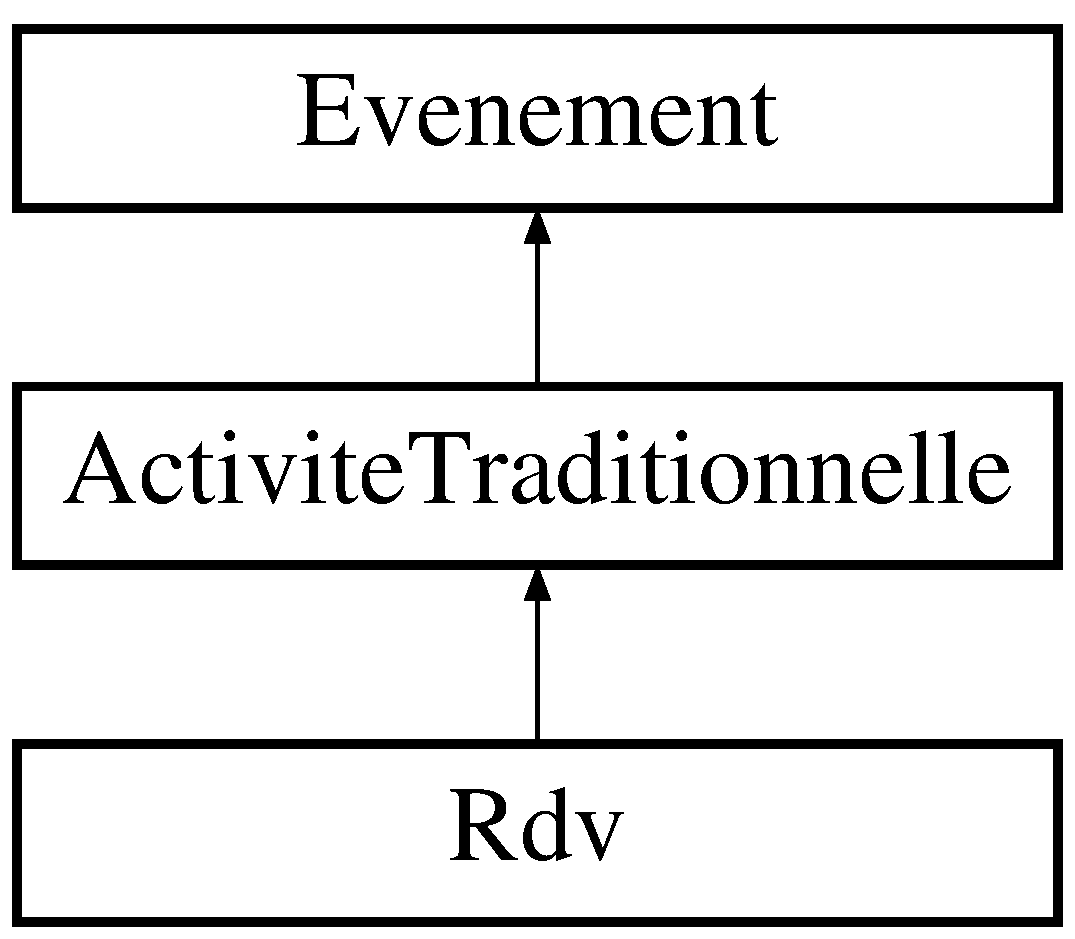
\includegraphics[height=3.000000cm]{class_rdv}
\end{center}
\end{figure}
\subsection*{Public Member Functions}
\begin{DoxyCompactItemize}
\item 
\hypertarget{class_rdv_a585f37d877d156d4491d39cbfe438e8a}{}{\bfseries Rdv} (Q\+String titre, \hyperlink{class_duree}{Duree} duree, Q\+String lieu, Q\+String interlocuteur)\label{class_rdv_a585f37d877d156d4491d39cbfe438e8a}

\item 
\hypertarget{class_rdv_a97231c0f56bdd957d32bd31918d9fce5}{}const Q\+String \& {\bfseries get\+Interlocuteur} () const \label{class_rdv_a97231c0f56bdd957d32bd31918d9fce5}

\item 
void \hyperlink{class_rdv_ac98a6180fddd005e1b364dbb0da2170a}{set\+Interlocuteur} (const Q\+String \&interl)
\begin{DoxyCompactList}\small\item\em modifie l\textquotesingle{}interlocuteur \end{DoxyCompactList}\end{DoxyCompactItemize}
\subsection*{Private Attributes}
\begin{DoxyCompactItemize}
\item 
\hypertarget{class_rdv_a102377cc114da4bc1ad38771d9ed18d5}{}Q\+String {\bfseries interlocuteur}\label{class_rdv_a102377cc114da4bc1ad38771d9ed18d5}

\end{DoxyCompactItemize}
\subsection*{Additional Inherited Members}


\subsection{Detailed Description}
sert pour un rendez-\/vous (un seul interlocuteur) 

\subsection{Member Function Documentation}
\hypertarget{class_rdv_ac98a6180fddd005e1b364dbb0da2170a}{}\index{Rdv@{Rdv}!set\+Interlocuteur@{set\+Interlocuteur}}
\index{set\+Interlocuteur@{set\+Interlocuteur}!Rdv@{Rdv}}
\subsubsection[{set\+Interlocuteur}]{\setlength{\rightskip}{0pt plus 5cm}void Rdv\+::set\+Interlocuteur (
\begin{DoxyParamCaption}
\item[{const Q\+String \&}]{interl}
\end{DoxyParamCaption}
)\hspace{0.3cm}{\ttfamily [inline]}}\label{class_rdv_ac98a6180fddd005e1b364dbb0da2170a}


modifie l\textquotesingle{}interlocuteur 


\begin{DoxyParams}{Parameters}
{\em interl} & \+: nouvelle interlocuteur \\
\hline
\end{DoxyParams}


The documentation for this class was generated from the following file\+:\begin{DoxyCompactItemize}
\item 
C\+:/\+Users/\+Fixe/\+Desktop/\+Programmation/\+P\+R\+O\+J\+E\+T\+\_\+\+L\+O21/\+Projet/evenement.\+h\end{DoxyCompactItemize}

\hypertarget{class_reunion}{}\section{Reunion Class Reference}
\label{class_reunion}\index{Reunion@{Reunion}}


classe servant pour les activites avec plusieurss participants  




{\ttfamily \#include $<$evenement.\+h$>$}

Inheritance diagram for Reunion\+:\begin{figure}[H]
\begin{center}
\leavevmode
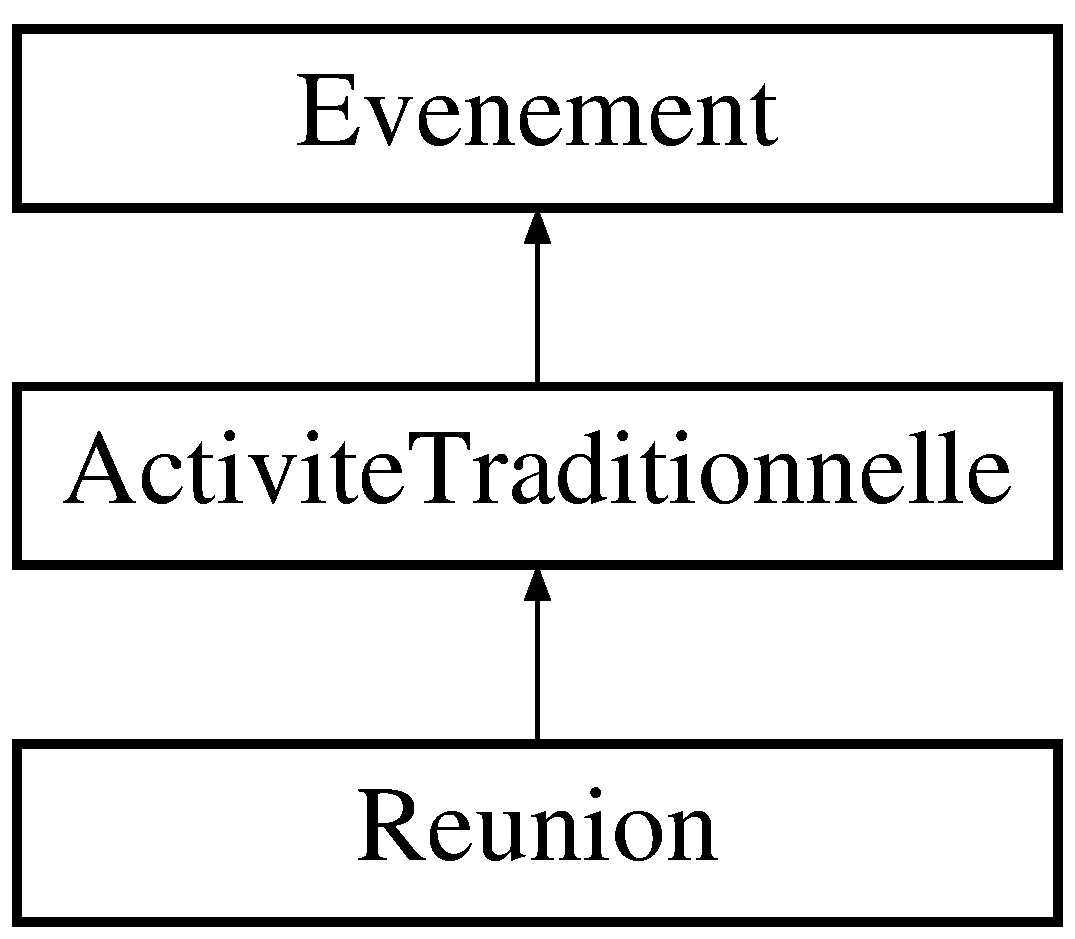
\includegraphics[height=3.000000cm]{class_reunion}
\end{center}
\end{figure}
\subsection*{Public Member Functions}
\begin{DoxyCompactItemize}
\item 
\hypertarget{class_reunion_a61af96d205195878e6ff2591907277c2}{}{\bfseries Reunion} (Q\+String titre, \hyperlink{class_duree}{Duree} duree, Q\+String lieu, std\+::vector$<$ Q\+String $>$ participants)\label{class_reunion_a61af96d205195878e6ff2591907277c2}

\item 
\hypertarget{class_reunion_a0b3ed32080ea2aa1f35ace3de8782f65}{}int {\bfseries get\+Nb\+Participants} ()\label{class_reunion_a0b3ed32080ea2aa1f35ace3de8782f65}

\item 
\hypertarget{class_reunion_ae4d5f04c6bb8c6e3aaa561ff40c86bb3}{}const std\+::vector$<$ Q\+String $>$ \& {\bfseries get\+Participants} () const \label{class_reunion_ae4d5f04c6bb8c6e3aaa561ff40c86bb3}

\item 
void \hyperlink{class_reunion_ac7af0e1d56757f6f0f55bf9526d4b45b}{ajouter\+Participant} (const Q\+String \&parti)
\begin{DoxyCompactList}\small\item\em rajoute le participant a la reunion \end{DoxyCompactList}\item 
void \hyperlink{class_reunion_a08293ef8675efe4035fca87fe2c4e6cb}{set\+Participants} (const std\+::vector$<$ Q\+String $>$ \&parti)
\begin{DoxyCompactList}\small\item\em remplace tous les participants \end{DoxyCompactList}\item 
void \hyperlink{class_reunion_a1b27209e80dd8a68fb87daa9526ebcaf}{supprimmer\+Participant} (const Q\+String \&parti)
\begin{DoxyCompactList}\small\item\em supprimme le participant désigné \end{DoxyCompactList}\end{DoxyCompactItemize}
\subsection*{Private Attributes}
\begin{DoxyCompactItemize}
\item 
\hypertarget{class_reunion_ad8ea8eb1f8f5e2edee4c12114e8b463d}{}std\+::vector$<$ Q\+String $>$ {\bfseries participants}\label{class_reunion_ad8ea8eb1f8f5e2edee4c12114e8b463d}

\end{DoxyCompactItemize}
\subsection*{Additional Inherited Members}


\subsection{Detailed Description}
classe servant pour les activites avec plusieurss participants 

\subsection{Member Function Documentation}
\hypertarget{class_reunion_ac7af0e1d56757f6f0f55bf9526d4b45b}{}\index{Reunion@{Reunion}!ajouter\+Participant@{ajouter\+Participant}}
\index{ajouter\+Participant@{ajouter\+Participant}!Reunion@{Reunion}}
\subsubsection[{ajouter\+Participant}]{\setlength{\rightskip}{0pt plus 5cm}void Reunion\+::ajouter\+Participant (
\begin{DoxyParamCaption}
\item[{const Q\+String \&}]{parti}
\end{DoxyParamCaption}
)\hspace{0.3cm}{\ttfamily [inline]}}\label{class_reunion_ac7af0e1d56757f6f0f55bf9526d4b45b}


rajoute le participant a la reunion 


\begin{DoxyParams}{Parameters}
{\em parti} & \+: participanta ajouter \\
\hline
\end{DoxyParams}
\hypertarget{class_reunion_a08293ef8675efe4035fca87fe2c4e6cb}{}\index{Reunion@{Reunion}!set\+Participants@{set\+Participants}}
\index{set\+Participants@{set\+Participants}!Reunion@{Reunion}}
\subsubsection[{set\+Participants}]{\setlength{\rightskip}{0pt plus 5cm}void Reunion\+::set\+Participants (
\begin{DoxyParamCaption}
\item[{const std\+::vector$<$ Q\+String $>$ \&}]{parti}
\end{DoxyParamCaption}
)}\label{class_reunion_a08293ef8675efe4035fca87fe2c4e6cb}


remplace tous les participants 


\begin{DoxyParams}{Parameters}
{\em parti} & \+: nouveaux participants \\
\hline
\end{DoxyParams}
\hypertarget{class_reunion_a1b27209e80dd8a68fb87daa9526ebcaf}{}\index{Reunion@{Reunion}!supprimmer\+Participant@{supprimmer\+Participant}}
\index{supprimmer\+Participant@{supprimmer\+Participant}!Reunion@{Reunion}}
\subsubsection[{supprimmer\+Participant}]{\setlength{\rightskip}{0pt plus 5cm}void Reunion\+::supprimmer\+Participant (
\begin{DoxyParamCaption}
\item[{const Q\+String \&}]{parti}
\end{DoxyParamCaption}
)}\label{class_reunion_a1b27209e80dd8a68fb87daa9526ebcaf}


supprimme le participant désigné 


\begin{DoxyParams}{Parameters}
{\em parti} & \+: participants a supprimmer \\
\hline
\end{DoxyParams}


The documentation for this class was generated from the following files\+:\begin{DoxyCompactItemize}
\item 
C\+:/\+Users/\+Fixe/\+Desktop/\+Programmation/\+P\+R\+O\+J\+E\+T\+\_\+\+L\+O21/\+Projet/evenement.\+h\item 
C\+:/\+Users/\+Fixe/\+Desktop/\+Programmation/\+P\+R\+O\+J\+E\+T\+\_\+\+L\+O21/\+Projet/evenement.\+cpp\end{DoxyCompactItemize}

\hypertarget{class_tache}{}\section{Tache Class Reference}
\label{class_tache}\index{Tache@{Tache}}


Abstrait, herite \hyperlink{class_evenement}{Evenement} toutes les taches en héritent, unité de base d\textquotesingle{}un projet.  




{\ttfamily \#include $<$evenement.\+h$>$}

Inheritance diagram for Tache\+:\begin{figure}[H]
\begin{center}
\leavevmode
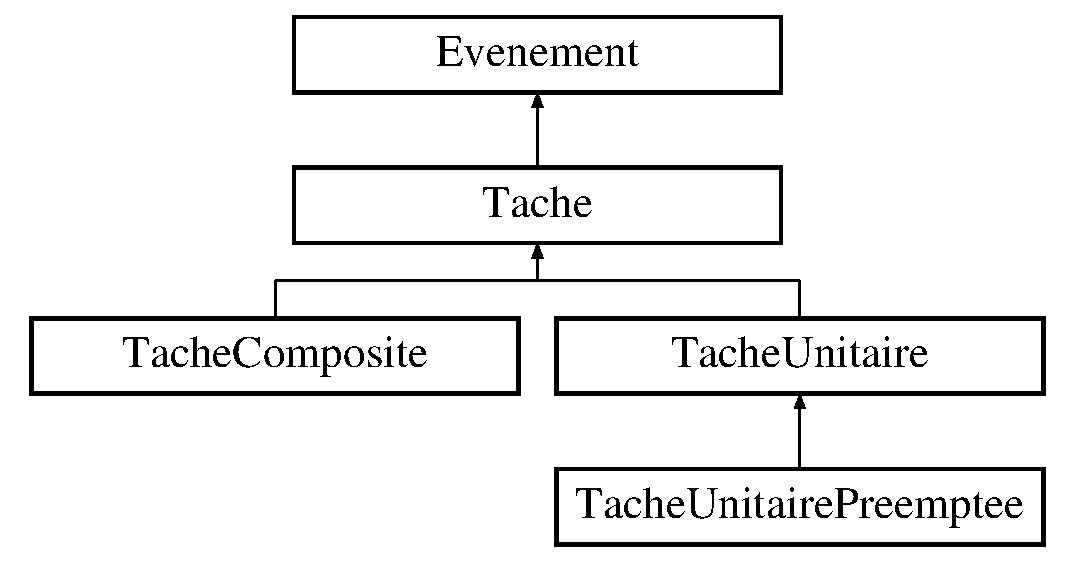
\includegraphics[height=4.000000cm]{class_tache}
\end{center}
\end{figure}
\subsection*{Public Member Functions}
\begin{DoxyCompactItemize}
\item 
virtual void \hyperlink{class_tache_a662db9ee24100a3d52853542c98dadf7}{set\+Programme} (bool effectue)
\begin{DoxyCompactList}\small\item\em reimplementation, permet de mettre a jour le statut de la \hyperlink{class_tache}{Tache} parente \end{DoxyCompactList}\item 
\hypertarget{class_tache_a49df0845676da96a48b0e229f45d4b08}{}const Q\+Date \& {\bfseries get\+Date\+Disponibilite} () const \label{class_tache_a49df0845676da96a48b0e229f45d4b08}

\item 
\hypertarget{class_tache_a77b8bb68047cae864ebeb19575fcfecd}{}const Q\+Date \& {\bfseries get\+Date\+Echeance} () const \label{class_tache_a77b8bb68047cae864ebeb19575fcfecd}

\item 
\hypertarget{class_tache_a8d3cb6f1e1adc46f938f4cab89e5218b}{}\hyperlink{class_tache}{Tache} $\ast$ {\bfseries get\+Parent} ()\label{class_tache_a8d3cb6f1e1adc46f938f4cab89e5218b}

\item 
\hypertarget{class_tache_a3ea1915199eeb501ed1c5cd871992dd6}{}const \hyperlink{class_tache}{Tache} $\ast$ {\bfseries get\+Parent} () const \label{class_tache_a3ea1915199eeb501ed1c5cd871992dd6}

\item 
\hypertarget{class_tache_ae5f783fff550c19580e3de7c143eab9e}{}const std\+::vector$<$ \hyperlink{class_tache}{Tache} $\ast$ $>$ \& {\bfseries get\+Prerequis} () const \label{class_tache_ae5f783fff550c19580e3de7c143eab9e}

\item 
void \hyperlink{class_tache_af6f744073c271d1c8bd302d1f4a8723a}{set\+Parent} (\hyperlink{class_tache}{Tache} $\ast$n\+\_\+parent)
\begin{DoxyCompactList}\small\item\em modifie le parent \end{DoxyCompactList}\item 
void \hyperlink{class_tache_ad3c79deb07748c25b6d97474571febec}{ajout\+Prerequi} (\hyperlink{class_tache}{Tache} $\ast$pre)
\begin{DoxyCompactList}\small\item\em ajoute un prérequis, renvoit exception si probleme$>$ \end{DoxyCompactList}\item 
void \hyperlink{class_tache_a96bbd20d7dcbb38ce128038190a656cd}{del\+Prerequi} (\hyperlink{class_tache}{Tache} $\ast$pre)
\begin{DoxyCompactList}\small\item\em supprimme un prérequis, renvoit exception si probleme$>$ \end{DoxyCompactList}\item 
void \hyperlink{class_tache_a68b96ac5212ecb13d0923f79da857183}{ajout\+Prerequis} (std\+::vector$<$ \hyperlink{class_tache}{Tache} $\ast$ $>$ vec)
\begin{DoxyCompactList}\small\item\em ajoute une liste prérequis, renvoit exception si probleme$>$ \end{DoxyCompactList}\item 
void \hyperlink{class_tache_a0fa9ada5b4236a1fb4f8876c3d220c59}{set\+Prerequis} (std\+::vector$<$ \hyperlink{class_tache}{Tache} $\ast$ $>$ vec)
\begin{DoxyCompactList}\small\item\em remet a 0 les prerequis et ajoute les nouveaux$>$ renvoit exception et remets les prerequis a l\textquotesingle{}etat antérieur si nouveaux prerequis impossibles \end{DoxyCompactList}\item 
void \hyperlink{class_tache_ad12e97235d69bd52f3c00c0dad21a3cf}{set\+Date\+Disponibilite} (const Q\+Date \&d\+Dispo)
\begin{DoxyCompactList}\small\item\em modifie la date de disponibilite \end{DoxyCompactList}\item 
void \hyperlink{class_tache_a73c12eb28e5130e986b3e2909735f012}{set\+Date\+Echeance} (const Q\+Date \&d\+Echeance)
\begin{DoxyCompactList}\small\item\em modifie la date d\textquotesingle{}echeance \end{DoxyCompactList}\item 
void \hyperlink{class_tache_a40fdf3048f276628904c5da0c971e314}{set\+Dates\+Disponibilite\+Echeance} (const Q\+Date \&d\+Dispo, const Q\+Date \&d\+Echeance)
\begin{DoxyCompactList}\small\item\em modifie la date d\textquotesingle{}echeance et disponibilite \end{DoxyCompactList}\end{DoxyCompactItemize}
\subsection*{Protected Member Functions}
\begin{DoxyCompactItemize}
\item 
\hypertarget{class_tache_aefe43451eb0c8140f5bfab7b376ef4fe}{}{\bfseries Tache} (int id, const Q\+String \&titre, const Q\+Date \&d\+Dispo, const Q\+Date \&d\+Echeance, std\+::vector$<$ \hyperlink{class_tache}{Tache} $\ast$ $>$ prerequis=std\+::vector$<$ \hyperlink{class_tache}{Tache} $\ast$ $>$(), \hyperlink{class_tache}{Tache} $\ast$parent=0)\label{class_tache_aefe43451eb0c8140f5bfab7b376ef4fe}

\end{DoxyCompactItemize}
\subsection*{Private Attributes}
\begin{DoxyCompactItemize}
\item 
\hypertarget{class_tache_ac8758b826b1be639dad8bcb556659a36}{}Q\+Date {\bfseries date\+Dispo}\label{class_tache_ac8758b826b1be639dad8bcb556659a36}

\item 
\hypertarget{class_tache_a7671c127da40ae35075f069a64396f45}{}Q\+Date {\bfseries date\+Echeance}\label{class_tache_a7671c127da40ae35075f069a64396f45}

\item 
\hypertarget{class_tache_a272b3f2cf7cba4a1a7980063563f8b88}{}\hyperlink{class_tache}{Tache} $\ast$ {\bfseries parent}\label{class_tache_a272b3f2cf7cba4a1a7980063563f8b88}

\item 
\hypertarget{class_tache_ae1f847bb410d1c0b4c252d7add695ddf}{}std\+::vector$<$ \hyperlink{class_tache}{Tache} $\ast$ $>$ {\bfseries prerequis}\label{class_tache_ae1f847bb410d1c0b4c252d7add695ddf}

\end{DoxyCompactItemize}


\subsection{Detailed Description}
Abstrait, herite \hyperlink{class_evenement}{Evenement} toutes les taches en héritent, unité de base d\textquotesingle{}un projet. 

\subsection{Member Function Documentation}
\hypertarget{class_tache_ad3c79deb07748c25b6d97474571febec}{}\index{Tache@{Tache}!ajout\+Prerequi@{ajout\+Prerequi}}
\index{ajout\+Prerequi@{ajout\+Prerequi}!Tache@{Tache}}
\subsubsection[{ajout\+Prerequi}]{\setlength{\rightskip}{0pt plus 5cm}void Tache\+::ajout\+Prerequi (
\begin{DoxyParamCaption}
\item[{{\bf Tache} $\ast$}]{pre}
\end{DoxyParamCaption}
)}\label{class_tache_ad3c79deb07748c25b6d97474571febec}


ajoute un prérequis, renvoit exception si probleme$>$ 

verifier si pas de boucles ou appartient prerequis


\begin{DoxyParams}{Parameters}
{\em pre} & \+: prerequis a ajouter \\
\hline
\end{DoxyParams}
\hypertarget{class_tache_a68b96ac5212ecb13d0923f79da857183}{}\index{Tache@{Tache}!ajout\+Prerequis@{ajout\+Prerequis}}
\index{ajout\+Prerequis@{ajout\+Prerequis}!Tache@{Tache}}
\subsubsection[{ajout\+Prerequis}]{\setlength{\rightskip}{0pt plus 5cm}void Tache\+::ajout\+Prerequis (
\begin{DoxyParamCaption}
\item[{std\+::vector$<$ {\bf Tache} $\ast$ $>$}]{vec}
\end{DoxyParamCaption}
)}\label{class_tache_a68b96ac5212ecb13d0923f79da857183}


ajoute une liste prérequis, renvoit exception si probleme$>$ 


\begin{DoxyParams}{Parameters}
{\em vec} & \+: prerequis a ajouter \\
\hline
\end{DoxyParams}
\hypertarget{class_tache_a96bbd20d7dcbb38ce128038190a656cd}{}\index{Tache@{Tache}!del\+Prerequi@{del\+Prerequi}}
\index{del\+Prerequi@{del\+Prerequi}!Tache@{Tache}}
\subsubsection[{del\+Prerequi}]{\setlength{\rightskip}{0pt plus 5cm}void Tache\+::del\+Prerequi (
\begin{DoxyParamCaption}
\item[{{\bf Tache} $\ast$}]{pre}
\end{DoxyParamCaption}
)}\label{class_tache_a96bbd20d7dcbb38ce128038190a656cd}


supprimme un prérequis, renvoit exception si probleme$>$ 


\begin{DoxyParams}{Parameters}
{\em pre} & \+: prerequis a supprimmer \\
\hline
\end{DoxyParams}
\hypertarget{class_tache_ad12e97235d69bd52f3c00c0dad21a3cf}{}\index{Tache@{Tache}!set\+Date\+Disponibilite@{set\+Date\+Disponibilite}}
\index{set\+Date\+Disponibilite@{set\+Date\+Disponibilite}!Tache@{Tache}}
\subsubsection[{set\+Date\+Disponibilite}]{\setlength{\rightskip}{0pt plus 5cm}void Tache\+::set\+Date\+Disponibilite (
\begin{DoxyParamCaption}
\item[{const Q\+Date \&}]{d\+Dispo}
\end{DoxyParamCaption}
)}\label{class_tache_ad12e97235d69bd52f3c00c0dad21a3cf}


modifie la date de disponibilite 


\begin{DoxyParams}{Parameters}
{\em d\+Dispo} & \+: nouvelle date de disponibilite \\
\hline
\end{DoxyParams}
\hypertarget{class_tache_a73c12eb28e5130e986b3e2909735f012}{}\index{Tache@{Tache}!set\+Date\+Echeance@{set\+Date\+Echeance}}
\index{set\+Date\+Echeance@{set\+Date\+Echeance}!Tache@{Tache}}
\subsubsection[{set\+Date\+Echeance}]{\setlength{\rightskip}{0pt plus 5cm}void Tache\+::set\+Date\+Echeance (
\begin{DoxyParamCaption}
\item[{const Q\+Date \&}]{d\+Echeance}
\end{DoxyParamCaption}
)}\label{class_tache_a73c12eb28e5130e986b3e2909735f012}


modifie la date d\textquotesingle{}echeance 


\begin{DoxyParams}{Parameters}
{\em d\+Echeance} & \+: nouvelle date d\textquotesingle{}echeance \\
\hline
\end{DoxyParams}
\hypertarget{class_tache_a40fdf3048f276628904c5da0c971e314}{}\index{Tache@{Tache}!set\+Dates\+Disponibilite\+Echeance@{set\+Dates\+Disponibilite\+Echeance}}
\index{set\+Dates\+Disponibilite\+Echeance@{set\+Dates\+Disponibilite\+Echeance}!Tache@{Tache}}
\subsubsection[{set\+Dates\+Disponibilite\+Echeance}]{\setlength{\rightskip}{0pt plus 5cm}void Tache\+::set\+Dates\+Disponibilite\+Echeance (
\begin{DoxyParamCaption}
\item[{const Q\+Date \&}]{d\+Dispo, }
\item[{const Q\+Date \&}]{d\+Echeance}
\end{DoxyParamCaption}
)}\label{class_tache_a40fdf3048f276628904c5da0c971e314}


modifie la date d\textquotesingle{}echeance et disponibilite 


\begin{DoxyParams}{Parameters}
{\em d\+Dispo} & \+: nouvelle date de disponibilite \\
\hline
{\em d\+Echeance} & \+: nouvelle date d\textquotesingle{}echeance \\
\hline
\end{DoxyParams}
\hypertarget{class_tache_af6f744073c271d1c8bd302d1f4a8723a}{}\index{Tache@{Tache}!set\+Parent@{set\+Parent}}
\index{set\+Parent@{set\+Parent}!Tache@{Tache}}
\subsubsection[{set\+Parent}]{\setlength{\rightskip}{0pt plus 5cm}void Tache\+::set\+Parent (
\begin{DoxyParamCaption}
\item[{{\bf Tache} $\ast$}]{n\+\_\+parent}
\end{DoxyParamCaption}
)}\label{class_tache_af6f744073c271d1c8bd302d1f4a8723a}


modifie le parent 


\begin{DoxyParams}{Parameters}
{\em n\+\_\+parent} & \+: nouveau parent de la tache \\
\hline
\end{DoxyParams}
\hypertarget{class_tache_a0fa9ada5b4236a1fb4f8876c3d220c59}{}\index{Tache@{Tache}!set\+Prerequis@{set\+Prerequis}}
\index{set\+Prerequis@{set\+Prerequis}!Tache@{Tache}}
\subsubsection[{set\+Prerequis}]{\setlength{\rightskip}{0pt plus 5cm}void Tache\+::set\+Prerequis (
\begin{DoxyParamCaption}
\item[{std\+::vector$<$ {\bf Tache} $\ast$ $>$}]{vec}
\end{DoxyParamCaption}
)}\label{class_tache_a0fa9ada5b4236a1fb4f8876c3d220c59}


remet a 0 les prerequis et ajoute les nouveaux$>$ renvoit exception et remets les prerequis a l\textquotesingle{}etat antérieur si nouveaux prerequis impossibles 


\begin{DoxyParams}{Parameters}
{\em vec} & \+: prerequis a ajouter \\
\hline
\end{DoxyParams}
\hypertarget{class_tache_a662db9ee24100a3d52853542c98dadf7}{}\index{Tache@{Tache}!set\+Programme@{set\+Programme}}
\index{set\+Programme@{set\+Programme}!Tache@{Tache}}
\subsubsection[{set\+Programme}]{\setlength{\rightskip}{0pt plus 5cm}void Tache\+::set\+Programme (
\begin{DoxyParamCaption}
\item[{bool}]{effectue}
\end{DoxyParamCaption}
)\hspace{0.3cm}{\ttfamily [virtual]}}\label{class_tache_a662db9ee24100a3d52853542c98dadf7}


reimplementation, permet de mettre a jour le statut de la \hyperlink{class_tache}{Tache} parente 


\begin{DoxyParams}{Parameters}
{\em effectue} & \+: dis si l\textquotesingle{}activite est programmée ou non \\
\hline
\end{DoxyParams}


Reimplemented from \hyperlink{class_evenement_ad4baf55b2e276b86ca5c5fd77c01f5d3}{Evenement}.



The documentation for this class was generated from the following files\+:\begin{DoxyCompactItemize}
\item 
C\+:/\+Users/\+Fixe/\+Desktop/\+Programmation/\+P\+R\+O\+J\+E\+T\+\_\+\+L\+O21/\+Projet/evenement.\+h\item 
C\+:/\+Users/\+Fixe/\+Desktop/\+Programmation/\+P\+R\+O\+J\+E\+T\+\_\+\+L\+O21/\+Projet/evenement.\+cpp\end{DoxyCompactItemize}

\hypertarget{class_tache_composite}{}\section{Tache\+Composite Class Reference}
\label{class_tache_composite}\index{Tache\+Composite@{Tache\+Composite}}


regroupement de taches \hyperlink{class_tache}{Tache} complexe, divisée en plusieurs sous Taches, agis comme un projet miniature  




{\ttfamily \#include $<$evenement.\+h$>$}

Inheritance diagram for Tache\+Composite\+:\begin{figure}[H]
\begin{center}
\leavevmode
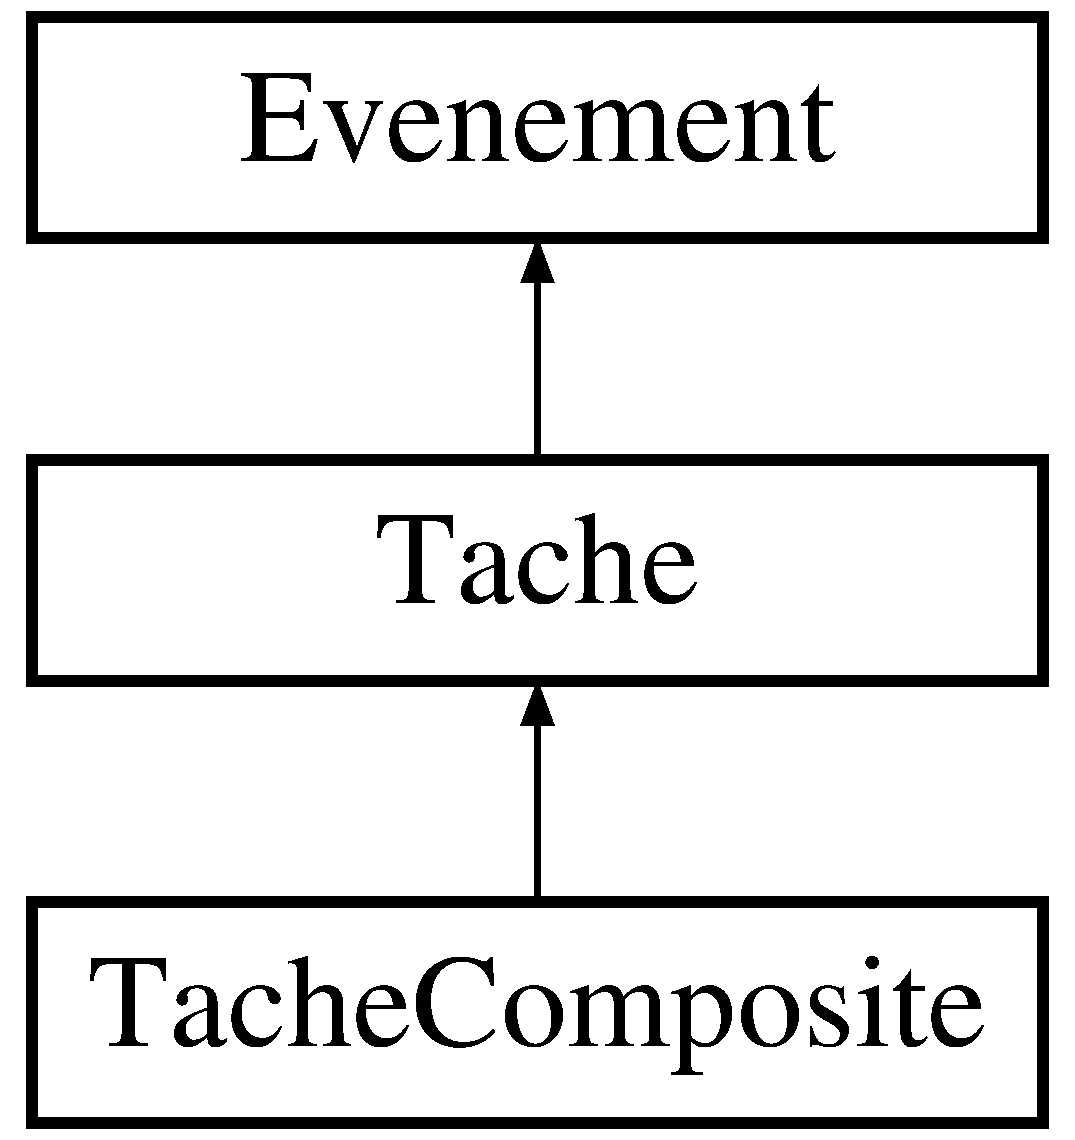
\includegraphics[height=3.000000cm]{class_tache_composite}
\end{center}
\end{figure}
\subsection*{Public Member Functions}
\begin{DoxyCompactItemize}
\item 
\hypertarget{class_tache_composite_ab7316533b8fbec7443a9ff2c33c69f86}{}void {\bfseries update\+Prog} ()\label{class_tache_composite_ab7316533b8fbec7443a9ff2c33c69f86}

\item 
void \hyperlink{class_tache_composite_a60c7332b9e4b6f162b9a4830b5260d33}{ajouter\+Sous\+Tache} (\hyperlink{class_tache}{Tache} $\ast$sous\+Tache)
\begin{DoxyCompactList}\small\item\em ajoute une sous tache deja créée \end{DoxyCompactList}\item 
void \hyperlink{class_tache_composite_a31b559ef0a8ec1eea5c7d68b11abd44a}{ajouter\+Sous\+Taches} (std\+::vector$<$ \hyperlink{class_tache}{Tache} $\ast$ $>$ ss\+Taches)
\begin{DoxyCompactList}\small\item\em ajoute un vecteur de sous tachse deja créées \end{DoxyCompactList}\item 
\hypertarget{class_tache_composite_ada263b48d9db1efae0bd77b43adf214a}{}const std\+::vector$<$ \hyperlink{class_tache}{Tache} $\ast$ $>$ \& {\bfseries get\+Sous\+Taches} () const \label{class_tache_composite_ada263b48d9db1efae0bd77b43adf214a}

\item 
const \hyperlink{class_tache}{Tache} \& \hyperlink{class_tache_composite_a8845d2b31a52770fbfc5fd309edb51eb}{get\+Sous\+Tache} (const Q\+String \&titre\+Sous\+Tache)
\begin{DoxyCompactList}\small\item\em renvoit une reference sur la sous tache en fonction de son titre \end{DoxyCompactList}\item 
const \hyperlink{class_tache}{Tache} \& \hyperlink{class_tache_composite_ac5a3b0618dd26d26509d1bc9db8a41b7}{get\+Sous\+Tache} (int id\+Sous\+Tache)
\begin{DoxyCompactList}\small\item\em renvoit une reference sur la sous tache en fonction de son id \end{DoxyCompactList}\item 
void \hyperlink{class_tache_composite_ac1f585bd7492034a7968f24ae28b47df}{supprimer\+Sous\+Tache} (int id\+Sous\+Tache)
\begin{DoxyCompactList}\small\item\em supprimme(seulement du vecteur) une sous tache en fonction de son titre \end{DoxyCompactList}\item 
void \hyperlink{class_tache_composite_a492a7906ff0437f406213206c1425c7e}{supprimer\+Sous\+Tache} (const Q\+String \&titre\+Sous\+Tache)
\begin{DoxyCompactList}\small\item\em supprimme(seulement du vecteur) une sous tache en fonction de son id \end{DoxyCompactList}\item 
\hypertarget{class_tache_composite_a2731407832e1ce44ec39ee4296f10aef}{}virtual \hyperlink{class_duree}{Duree} \hyperlink{class_tache_composite_a2731407832e1ce44ec39ee4296f10aef}{get\+Duree} () const \label{class_tache_composite_a2731407832e1ce44ec39ee4296f10aef}

\begin{DoxyCompactList}\small\item\em renvoit la durée de l\textquotesingle{}evenement la classe evenement ne contient pas d\textquotesingle{}attribut Durée, mais toutes ses sous classes (sauf tache Composite) en possèdent, on décide donc de la créer virtuelle pure \end{DoxyCompactList}\end{DoxyCompactItemize}
\subsection*{Protected Member Functions}
\begin{DoxyCompactItemize}
\item 
\hyperlink{class_tache_composite_afb044dffd39c4c4378bcd2ea9cfa4fa7}{Tache\+Composite} (int id, const Q\+String \&titre, const Q\+Date \&d\+Dispo, const Q\+Date \&d\+Echeance, std\+::vector$<$ \hyperlink{class_tache}{Tache} $\ast$ $>$ pre, \hyperlink{class_tache}{Tache} $\ast$parent)
\begin{DoxyCompactList}\small\item\em constructeur, accessible par sous classes et \hyperlink{class_projet}{Projet} \end{DoxyCompactList}\item 
\hyperlink{class_tache_composite_a7dd6c584f8fb36f9671df59c8971709e}{Tache\+Composite} (\hyperlink{class_tache_composite}{Tache\+Composite} \&other)
\begin{DoxyCompactList}\small\item\em constructeur par recopie, accessible par sous classes et \hyperlink{class_projet}{Projet} \end{DoxyCompactList}\item 
\hyperlink{class_tache_composite}{Tache\+Composite} \& \hyperlink{class_tache_composite_a4ddf7c1bfa9ef2e2790d5cef803172c8}{operator=} (\hyperlink{class_tache_composite}{Tache\+Composite} \&other)
\begin{DoxyCompactList}\small\item\em operateur d\textquotesingle{}affectation, accessible par sous classes et \hyperlink{class_projet}{Projet} \end{DoxyCompactList}\end{DoxyCompactItemize}
\subsection*{Private Member Functions}
\begin{DoxyCompactItemize}
\item 
\hyperlink{class_tache}{Tache} $\ast$ \hyperlink{class_tache_composite_a0cb50cd658968c93e255f5f55dddd884}{trouver\+Sous\+Tache} (const Q\+String \&titre\+Sous\+Tache) const 
\begin{DoxyCompactList}\small\item\em renvoit lun pointeur sur la sous tache en fonction de son titre \end{DoxyCompactList}\item 
\hyperlink{class_tache}{Tache} $\ast$ \hyperlink{class_tache_composite_a4257d0b5cdd8a9d54307ea55366bf692}{trouver\+Sous\+Tache} (int id\+Sous\+Tache) const 
\begin{DoxyCompactList}\small\item\em renvoit un pointeur sur la sous tache en fonction de son id \end{DoxyCompactList}\end{DoxyCompactItemize}
\subsection*{Private Attributes}
\begin{DoxyCompactItemize}
\item 
\hypertarget{class_tache_composite_aa57ff208216ab0a2488ef9ad464da6c1}{}std\+::vector$<$ \hyperlink{class_tache}{Tache} $\ast$ $>$ {\bfseries sous\+Taches}\label{class_tache_composite_aa57ff208216ab0a2488ef9ad464da6c1}

\end{DoxyCompactItemize}
\subsection*{Friends}
\begin{DoxyCompactItemize}
\item 
\hypertarget{class_tache_composite_ab87b41c3faa36955cc370972f5cce344}{}class {\bfseries Projet}\label{class_tache_composite_ab87b41c3faa36955cc370972f5cce344}

\end{DoxyCompactItemize}


\subsection{Detailed Description}
regroupement de taches \hyperlink{class_tache}{Tache} complexe, divisée en plusieurs sous Taches, agis comme un projet miniature 

\subsection{Constructor \& Destructor Documentation}
\hypertarget{class_tache_composite_afb044dffd39c4c4378bcd2ea9cfa4fa7}{}\index{Tache\+Composite@{Tache\+Composite}!Tache\+Composite@{Tache\+Composite}}
\index{Tache\+Composite@{Tache\+Composite}!Tache\+Composite@{Tache\+Composite}}
\subsubsection[{Tache\+Composite}]{\setlength{\rightskip}{0pt plus 5cm}Tache\+Composite\+::\+Tache\+Composite (
\begin{DoxyParamCaption}
\item[{int}]{id, }
\item[{const Q\+String \&}]{titre, }
\item[{const Q\+Date \&}]{d\+Dispo, }
\item[{const Q\+Date \&}]{d\+Echeance, }
\item[{std\+::vector$<$ {\bf Tache} $\ast$ $>$}]{pre, }
\item[{{\bf Tache} $\ast$}]{parent}
\end{DoxyParamCaption}
)\hspace{0.3cm}{\ttfamily [inline]}, {\ttfamily [protected]}}\label{class_tache_composite_afb044dffd39c4c4378bcd2ea9cfa4fa7}


constructeur, accessible par sous classes et \hyperlink{class_projet}{Projet} 


\begin{DoxyParams}{Parameters}
{\em other} & \+: tache Composite a recopier \\
\hline
\end{DoxyParams}
\hypertarget{class_tache_composite_a7dd6c584f8fb36f9671df59c8971709e}{}\index{Tache\+Composite@{Tache\+Composite}!Tache\+Composite@{Tache\+Composite}}
\index{Tache\+Composite@{Tache\+Composite}!Tache\+Composite@{Tache\+Composite}}
\subsubsection[{Tache\+Composite}]{\setlength{\rightskip}{0pt plus 5cm}Tache\+Composite\+::\+Tache\+Composite (
\begin{DoxyParamCaption}
\item[{{\bf Tache\+Composite} \&}]{other}
\end{DoxyParamCaption}
)\hspace{0.3cm}{\ttfamily [protected]}}\label{class_tache_composite_a7dd6c584f8fb36f9671df59c8971709e}


constructeur par recopie, accessible par sous classes et \hyperlink{class_projet}{Projet} 


\begin{DoxyParams}{Parameters}
{\em other} & \+: tache Composite a recopier \\
\hline
\end{DoxyParams}


\subsection{Member Function Documentation}
\hypertarget{class_tache_composite_a60c7332b9e4b6f162b9a4830b5260d33}{}\index{Tache\+Composite@{Tache\+Composite}!ajouter\+Sous\+Tache@{ajouter\+Sous\+Tache}}
\index{ajouter\+Sous\+Tache@{ajouter\+Sous\+Tache}!Tache\+Composite@{Tache\+Composite}}
\subsubsection[{ajouter\+Sous\+Tache}]{\setlength{\rightskip}{0pt plus 5cm}void Tache\+Composite\+::ajouter\+Sous\+Tache (
\begin{DoxyParamCaption}
\item[{{\bf Tache} $\ast$}]{sous\+Tache}
\end{DoxyParamCaption}
)}\label{class_tache_composite_a60c7332b9e4b6f162b9a4830b5260d33}


ajoute une sous tache deja créée 


\begin{DoxyParams}{Parameters}
{\em sous\+Tache} & \+: sous tache a ajouter \\
\hline
\end{DoxyParams}
\hypertarget{class_tache_composite_a31b559ef0a8ec1eea5c7d68b11abd44a}{}\index{Tache\+Composite@{Tache\+Composite}!ajouter\+Sous\+Taches@{ajouter\+Sous\+Taches}}
\index{ajouter\+Sous\+Taches@{ajouter\+Sous\+Taches}!Tache\+Composite@{Tache\+Composite}}
\subsubsection[{ajouter\+Sous\+Taches}]{\setlength{\rightskip}{0pt plus 5cm}void Tache\+Composite\+::ajouter\+Sous\+Taches (
\begin{DoxyParamCaption}
\item[{std\+::vector$<$ {\bf Tache} $\ast$ $>$}]{ss\+Taches}
\end{DoxyParamCaption}
)}\label{class_tache_composite_a31b559ef0a8ec1eea5c7d68b11abd44a}


ajoute un vecteur de sous tachse deja créées 


\begin{DoxyParams}{Parameters}
{\em ss\+Taches} & \+: sous taches a ajouter \\
\hline
\end{DoxyParams}
\hypertarget{class_tache_composite_a8845d2b31a52770fbfc5fd309edb51eb}{}\index{Tache\+Composite@{Tache\+Composite}!get\+Sous\+Tache@{get\+Sous\+Tache}}
\index{get\+Sous\+Tache@{get\+Sous\+Tache}!Tache\+Composite@{Tache\+Composite}}
\subsubsection[{get\+Sous\+Tache}]{\setlength{\rightskip}{0pt plus 5cm}const {\bf Tache} \& Tache\+Composite\+::get\+Sous\+Tache (
\begin{DoxyParamCaption}
\item[{const Q\+String \&}]{titre\+Sous\+Tache}
\end{DoxyParamCaption}
)}\label{class_tache_composite_a8845d2b31a52770fbfc5fd309edb51eb}


renvoit une reference sur la sous tache en fonction de son titre 


\begin{DoxyParams}{Parameters}
{\em titre\+Sous\+Tache} & \+: titre recherche \\
\hline
\end{DoxyParams}
\hypertarget{class_tache_composite_ac5a3b0618dd26d26509d1bc9db8a41b7}{}\index{Tache\+Composite@{Tache\+Composite}!get\+Sous\+Tache@{get\+Sous\+Tache}}
\index{get\+Sous\+Tache@{get\+Sous\+Tache}!Tache\+Composite@{Tache\+Composite}}
\subsubsection[{get\+Sous\+Tache}]{\setlength{\rightskip}{0pt plus 5cm}const {\bf Tache} \& Tache\+Composite\+::get\+Sous\+Tache (
\begin{DoxyParamCaption}
\item[{int}]{id\+Sous\+Tache}
\end{DoxyParamCaption}
)}\label{class_tache_composite_ac5a3b0618dd26d26509d1bc9db8a41b7}


renvoit une reference sur la sous tache en fonction de son id 


\begin{DoxyParams}{Parameters}
{\em id\+Sous\+Tache} & \+: id recherché \\
\hline
\end{DoxyParams}
\hypertarget{class_tache_composite_a4ddf7c1bfa9ef2e2790d5cef803172c8}{}\index{Tache\+Composite@{Tache\+Composite}!operator=@{operator=}}
\index{operator=@{operator=}!Tache\+Composite@{Tache\+Composite}}
\subsubsection[{operator=}]{\setlength{\rightskip}{0pt plus 5cm}{\bf Tache\+Composite} \& Tache\+Composite\+::operator= (
\begin{DoxyParamCaption}
\item[{{\bf Tache\+Composite} \&}]{other}
\end{DoxyParamCaption}
)\hspace{0.3cm}{\ttfamily [protected]}}\label{class_tache_composite_a4ddf7c1bfa9ef2e2790d5cef803172c8}


operateur d\textquotesingle{}affectation, accessible par sous classes et \hyperlink{class_projet}{Projet} 


\begin{DoxyParams}{Parameters}
{\em other} & \+: tache Composite a recopier \\
\hline
\end{DoxyParams}
\hypertarget{class_tache_composite_ac1f585bd7492034a7968f24ae28b47df}{}\index{Tache\+Composite@{Tache\+Composite}!supprimer\+Sous\+Tache@{supprimer\+Sous\+Tache}}
\index{supprimer\+Sous\+Tache@{supprimer\+Sous\+Tache}!Tache\+Composite@{Tache\+Composite}}
\subsubsection[{supprimer\+Sous\+Tache}]{\setlength{\rightskip}{0pt plus 5cm}void Tache\+Composite\+::supprimer\+Sous\+Tache (
\begin{DoxyParamCaption}
\item[{int}]{id\+Sous\+Tache}
\end{DoxyParamCaption}
)}\label{class_tache_composite_ac1f585bd7492034a7968f24ae28b47df}


supprimme(seulement du vecteur) une sous tache en fonction de son titre 


\begin{DoxyParams}{Parameters}
{\em id\+Sous\+Tache} & \+: id recherché \\
\hline
\end{DoxyParams}
\hypertarget{class_tache_composite_a492a7906ff0437f406213206c1425c7e}{}\index{Tache\+Composite@{Tache\+Composite}!supprimer\+Sous\+Tache@{supprimer\+Sous\+Tache}}
\index{supprimer\+Sous\+Tache@{supprimer\+Sous\+Tache}!Tache\+Composite@{Tache\+Composite}}
\subsubsection[{supprimer\+Sous\+Tache}]{\setlength{\rightskip}{0pt plus 5cm}void Tache\+Composite\+::supprimer\+Sous\+Tache (
\begin{DoxyParamCaption}
\item[{const Q\+String \&}]{titre\+Sous\+Tache}
\end{DoxyParamCaption}
)}\label{class_tache_composite_a492a7906ff0437f406213206c1425c7e}


supprimme(seulement du vecteur) une sous tache en fonction de son id 


\begin{DoxyParams}{Parameters}
{\em titre\+Sous\+Tache} & \+: titre recherché \\
\hline
\end{DoxyParams}
\hypertarget{class_tache_composite_a0cb50cd658968c93e255f5f55dddd884}{}\index{Tache\+Composite@{Tache\+Composite}!trouver\+Sous\+Tache@{trouver\+Sous\+Tache}}
\index{trouver\+Sous\+Tache@{trouver\+Sous\+Tache}!Tache\+Composite@{Tache\+Composite}}
\subsubsection[{trouver\+Sous\+Tache}]{\setlength{\rightskip}{0pt plus 5cm}{\bf Tache} $\ast$ Tache\+Composite\+::trouver\+Sous\+Tache (
\begin{DoxyParamCaption}
\item[{const Q\+String \&}]{titre\+Sous\+Tache}
\end{DoxyParamCaption}
) const\hspace{0.3cm}{\ttfamily [private]}}\label{class_tache_composite_a0cb50cd658968c93e255f5f55dddd884}


renvoit lun pointeur sur la sous tache en fonction de son titre 


\begin{DoxyParams}{Parameters}
{\em titre\+Sous\+Tache} & \+: titre recherché \\
\hline
\end{DoxyParams}
\hypertarget{class_tache_composite_a4257d0b5cdd8a9d54307ea55366bf692}{}\index{Tache\+Composite@{Tache\+Composite}!trouver\+Sous\+Tache@{trouver\+Sous\+Tache}}
\index{trouver\+Sous\+Tache@{trouver\+Sous\+Tache}!Tache\+Composite@{Tache\+Composite}}
\subsubsection[{trouver\+Sous\+Tache}]{\setlength{\rightskip}{0pt plus 5cm}{\bf Tache} $\ast$ Tache\+Composite\+::trouver\+Sous\+Tache (
\begin{DoxyParamCaption}
\item[{int}]{id\+Sous\+Tache}
\end{DoxyParamCaption}
) const\hspace{0.3cm}{\ttfamily [private]}}\label{class_tache_composite_a4257d0b5cdd8a9d54307ea55366bf692}


renvoit un pointeur sur la sous tache en fonction de son id 


\begin{DoxyParams}{Parameters}
{\em id\+Sous\+Tache} & \+: id recherché \\
\hline
\end{DoxyParams}


The documentation for this class was generated from the following files\+:\begin{DoxyCompactItemize}
\item 
C\+:/\+Users/\+Fixe/\+Desktop/\+Programmation/\+P\+R\+O\+J\+E\+T\+\_\+\+L\+O21/\+Projet/evenement.\+h\item 
C\+:/\+Users/\+Fixe/\+Desktop/\+Programmation/\+P\+R\+O\+J\+E\+T\+\_\+\+L\+O21/\+Projet/evenement.\+cpp\end{DoxyCompactItemize}

\hypertarget{class_tache_unitaire}{}\section{Tache\+Unitaire Class Reference}
\label{class_tache_unitaire}\index{Tache\+Unitaire@{Tache\+Unitaire}}


\hyperlink{class_tache}{Tache} simple tache simple, d\textquotesingle{}une certaine durée, a effectuer en une fois.  




{\ttfamily \#include $<$evenement.\+h$>$}

Inheritance diagram for Tache\+Unitaire\+:\begin{figure}[H]
\begin{center}
\leavevmode
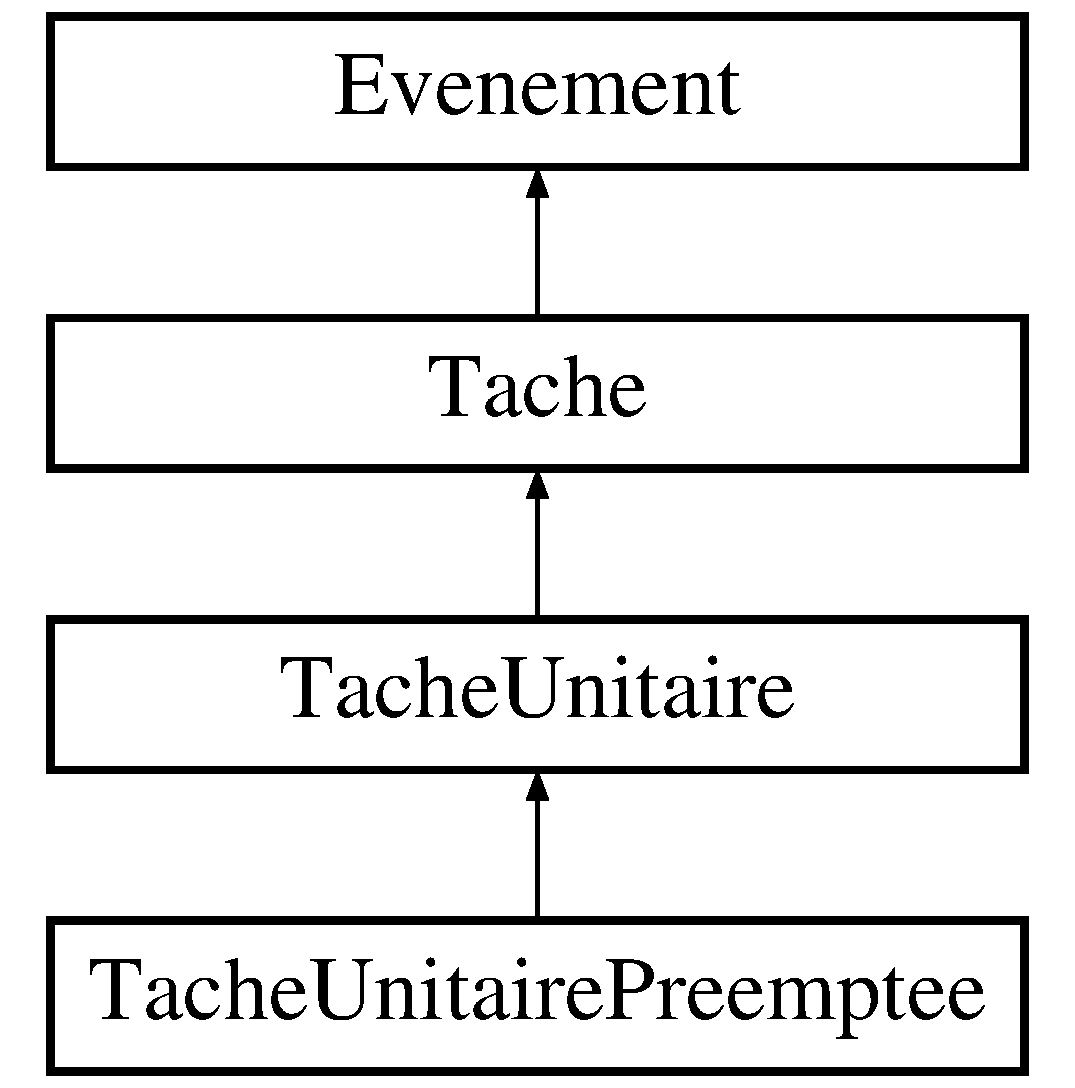
\includegraphics[height=4.000000cm]{class_tache_unitaire}
\end{center}
\end{figure}
\subsection*{Public Member Functions}
\begin{DoxyCompactItemize}
\item 
\hypertarget{class_tache_unitaire_aeea74499e37ea186a85edb21503a9758}{}virtual \hyperlink{class_duree}{Duree} \hyperlink{class_tache_unitaire_aeea74499e37ea186a85edb21503a9758}{get\+Duree} () const \label{class_tache_unitaire_aeea74499e37ea186a85edb21503a9758}

\begin{DoxyCompactList}\small\item\em renvoit la durée de l\textquotesingle{}evenement la classe evenement ne contient pas d\textquotesingle{}attribut Durée, mais toutes ses sous classes (sauf tache Composite) en possèdent, on décide donc de la créer virtuelle pure \end{DoxyCompactList}\item 
void \hyperlink{class_tache_unitaire_a4472e37f36d315d2e02fe8d743bc6616}{set\+Duree} (\hyperlink{class_duree}{Duree} \&nouvelle\+Duree)
\begin{DoxyCompactList}\small\item\em modifie la duree de la tache \end{DoxyCompactList}\end{DoxyCompactItemize}
\subsection*{Protected Member Functions}
\begin{DoxyCompactItemize}
\item 
\hypertarget{class_tache_unitaire_a7091788806d9ce59ba1f6b1dc1e3a92b}{}{\bfseries Tache\+Unitaire} (int id, const Q\+String \&titre, const Q\+Date \&d\+Dispo, const Q\+Date \&d\+Echeance, \hyperlink{class_duree}{Duree} duree, const std\+::vector$<$ \hyperlink{class_tache}{Tache} $\ast$ $>$ pre, \hyperlink{class_tache}{Tache} $\ast$parent)\label{class_tache_unitaire_a7091788806d9ce59ba1f6b1dc1e3a92b}

\end{DoxyCompactItemize}
\subsection*{Private Attributes}
\begin{DoxyCompactItemize}
\item 
\hypertarget{class_tache_unitaire_aca42cdc08900e1419b872c2261c220a5}{}\hyperlink{class_duree}{Duree} {\bfseries duree}\label{class_tache_unitaire_aca42cdc08900e1419b872c2261c220a5}

\end{DoxyCompactItemize}
\subsection*{Friends}
\begin{DoxyCompactItemize}
\item 
\hypertarget{class_tache_unitaire_ab87b41c3faa36955cc370972f5cce344}{}class {\bfseries Projet}\label{class_tache_unitaire_ab87b41c3faa36955cc370972f5cce344}

\end{DoxyCompactItemize}


\subsection{Detailed Description}
\hyperlink{class_tache}{Tache} simple tache simple, d\textquotesingle{}une certaine durée, a effectuer en une fois. 

\subsection{Member Function Documentation}
\hypertarget{class_tache_unitaire_a4472e37f36d315d2e02fe8d743bc6616}{}\index{Tache\+Unitaire@{Tache\+Unitaire}!set\+Duree@{set\+Duree}}
\index{set\+Duree@{set\+Duree}!Tache\+Unitaire@{Tache\+Unitaire}}
\subsubsection[{set\+Duree}]{\setlength{\rightskip}{0pt plus 5cm}void Tache\+Unitaire\+::set\+Duree (
\begin{DoxyParamCaption}
\item[{{\bf Duree} \&}]{nouvelle\+Duree}
\end{DoxyParamCaption}
)\hspace{0.3cm}{\ttfamily [inline]}}\label{class_tache_unitaire_a4472e37f36d315d2e02fe8d743bc6616}


modifie la duree de la tache 


\begin{DoxyParams}{Parameters}
{\em nouvelle\+Duree} & \+: nouvelle duree de l\textquotesingle{}activite \\
\hline
\end{DoxyParams}


The documentation for this class was generated from the following file\+:\begin{DoxyCompactItemize}
\item 
C\+:/\+Users/\+Fixe/\+Desktop/\+Programmation/\+P\+R\+O\+J\+E\+T\+\_\+\+L\+O21/\+Projet/evenement.\+h\end{DoxyCompactItemize}

\hypertarget{class_tache_unitaire_preemptee}{}\section{Tache\+Unitaire\+Preemptee Class Reference}
\label{class_tache_unitaire_preemptee}\index{Tache\+Unitaire\+Preemptee@{Tache\+Unitaire\+Preemptee}}


\hyperlink{class_tache}{Tache} Preemptee tache simple, mais faisable en plusieurs fois.  




{\ttfamily \#include $<$evenement.\+h$>$}

Inheritance diagram for Tache\+Unitaire\+Preemptee\+:\begin{figure}[H]
\begin{center}
\leavevmode
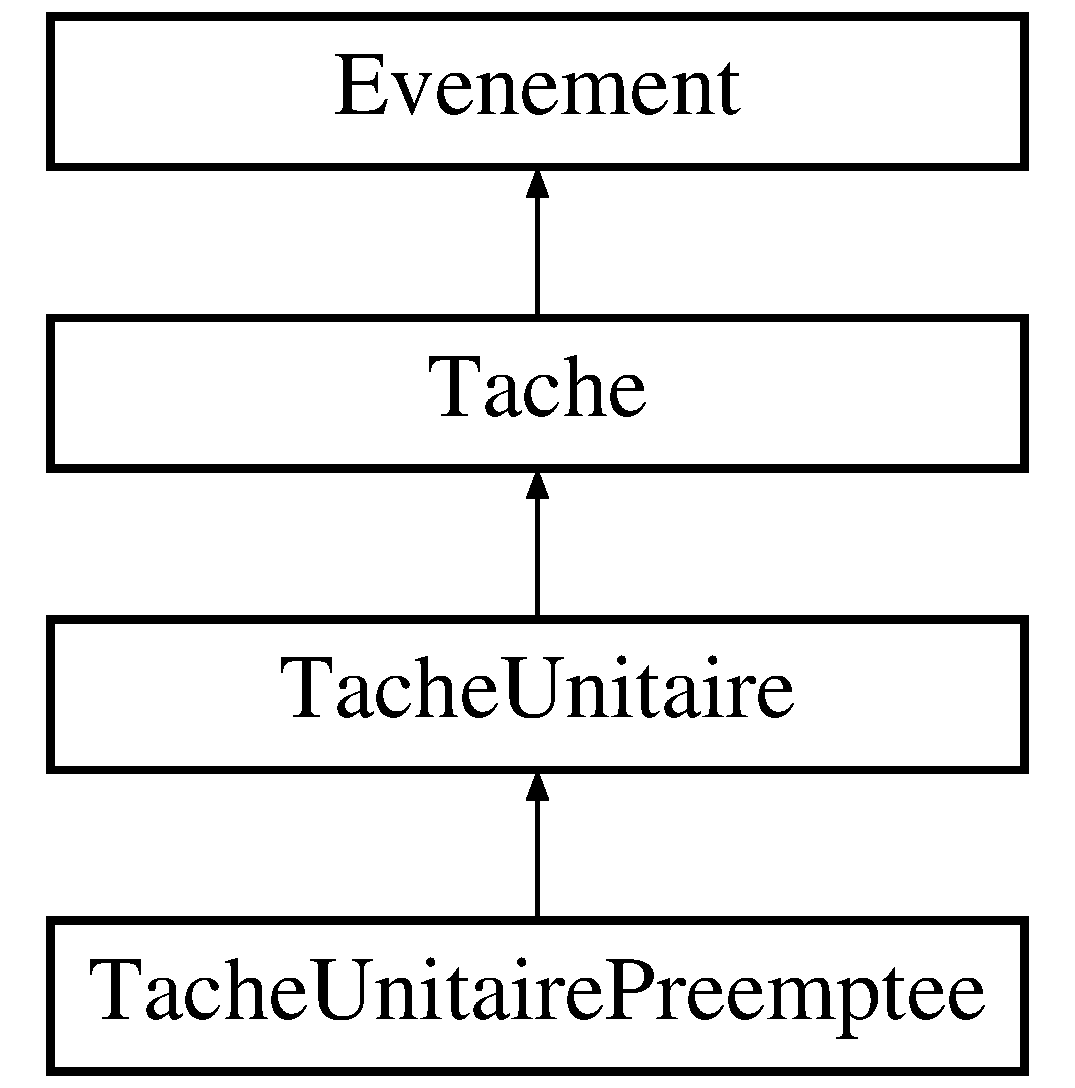
\includegraphics[height=4.000000cm]{class_tache_unitaire_preemptee}
\end{center}
\end{figure}
\subsection*{Public Member Functions}
\begin{DoxyCompactItemize}
\item 
void \hyperlink{class_tache_unitaire_preemptee_a4061516eb33059f302d5ebe1ad580e2d}{set\+Duree\+Effectuee} (const \hyperlink{class_duree}{Duree} \&d\+Effectuee)
\begin{DoxyCompactList}\small\item\em remets a zero la duree effectuee et rajoute celle en argument \end{DoxyCompactList}\item 
void \hyperlink{class_tache_unitaire_preemptee_af30a0fd0691b514d356321a45c57661c}{add\+Duree\+Effectuee} (const \hyperlink{class_duree}{Duree} \&d\+Effectuee)
\begin{DoxyCompactList}\small\item\em rajoute la duree effectuee \end{DoxyCompactList}\item 
void \hyperlink{class_tache_unitaire_preemptee_a1151a6443d9692a6a01f78dcb490aa4a}{sub\+Duree\+Effectuee} (const \hyperlink{class_duree}{Duree} \&d\+Supprimmee)
\begin{DoxyCompactList}\small\item\em enleve la duree non effectuee \end{DoxyCompactList}\item 
\hypertarget{class_tache_unitaire_preemptee_a9e2e18ad2e951c52fd66ab4a9e7937f7}{}const \hyperlink{class_duree}{Duree} \& {\bfseries get\+Duree\+Effectuee} () const \label{class_tache_unitaire_preemptee_a9e2e18ad2e951c52fd66ab4a9e7937f7}

\item 
\hypertarget{class_tache_unitaire_preemptee_a82eb73b30e1cfcbff1a15625637811b0}{}\hyperlink{class_duree}{Duree} {\bfseries get\+Duree\+Restante} () const \label{class_tache_unitaire_preemptee_a82eb73b30e1cfcbff1a15625637811b0}

\end{DoxyCompactItemize}
\subsection*{Protected Member Functions}
\begin{DoxyCompactItemize}
\item 
\hypertarget{class_tache_unitaire_preemptee_afdfea43ca79a7c1ea154499bbeb34af5}{}{\bfseries Tache\+Unitaire\+Preemptee} (int id, const Q\+String \&titre, const Q\+Date \&d\+Dispo, const Q\+Date \&d\+Echeance, \hyperlink{class_duree}{Duree} duree, const std\+::vector$<$ \hyperlink{class_tache}{Tache} $\ast$ $>$ pre, \hyperlink{class_tache}{Tache} $\ast$parent)\label{class_tache_unitaire_preemptee_afdfea43ca79a7c1ea154499bbeb34af5}

\end{DoxyCompactItemize}
\subsection*{Private Member Functions}
\begin{DoxyCompactItemize}
\item 
void \hyperlink{class_tache_unitaire_preemptee_ab3b4effe2c4d6a9bb1e63e4d177c1ef0}{check\+Possible} (std\+::string op, \hyperlink{class_duree}{Duree} d)
\begin{DoxyCompactList}\small\item\em verifie si la duree après opération est possible, renvoit exception si non \end{DoxyCompactList}\end{DoxyCompactItemize}
\subsection*{Private Attributes}
\begin{DoxyCompactItemize}
\item 
\hypertarget{class_tache_unitaire_preemptee_a73fdde2eeaff2f58445f1882aec44321}{}\hyperlink{class_duree}{Duree} {\bfseries duree\+Effectuee}\label{class_tache_unitaire_preemptee_a73fdde2eeaff2f58445f1882aec44321}

\end{DoxyCompactItemize}
\subsection*{Friends}
\begin{DoxyCompactItemize}
\item 
\hypertarget{class_tache_unitaire_preemptee_ab87b41c3faa36955cc370972f5cce344}{}class {\bfseries Projet}\label{class_tache_unitaire_preemptee_ab87b41c3faa36955cc370972f5cce344}

\end{DoxyCompactItemize}


\subsection{Detailed Description}
\hyperlink{class_tache}{Tache} Preemptee tache simple, mais faisable en plusieurs fois. 

\subsection{Member Function Documentation}
\hypertarget{class_tache_unitaire_preemptee_af30a0fd0691b514d356321a45c57661c}{}\index{Tache\+Unitaire\+Preemptee@{Tache\+Unitaire\+Preemptee}!add\+Duree\+Effectuee@{add\+Duree\+Effectuee}}
\index{add\+Duree\+Effectuee@{add\+Duree\+Effectuee}!Tache\+Unitaire\+Preemptee@{Tache\+Unitaire\+Preemptee}}
\subsubsection[{add\+Duree\+Effectuee}]{\setlength{\rightskip}{0pt plus 5cm}void Tache\+Unitaire\+Preemptee\+::add\+Duree\+Effectuee (
\begin{DoxyParamCaption}
\item[{const {\bf Duree} \&}]{d\+Effectuee}
\end{DoxyParamCaption}
)}\label{class_tache_unitaire_preemptee_af30a0fd0691b514d356321a45c57661c}


rajoute la duree effectuee 


\begin{DoxyParams}{Parameters}
{\em d\+Effectuee} & \+: duree a additionner \\
\hline
\end{DoxyParams}
\hypertarget{class_tache_unitaire_preemptee_ab3b4effe2c4d6a9bb1e63e4d177c1ef0}{}\index{Tache\+Unitaire\+Preemptee@{Tache\+Unitaire\+Preemptee}!check\+Possible@{check\+Possible}}
\index{check\+Possible@{check\+Possible}!Tache\+Unitaire\+Preemptee@{Tache\+Unitaire\+Preemptee}}
\subsubsection[{check\+Possible}]{\setlength{\rightskip}{0pt plus 5cm}void Tache\+Unitaire\+Preemptee\+::check\+Possible (
\begin{DoxyParamCaption}
\item[{std\+::string}]{op, }
\item[{{\bf Duree}}]{d}
\end{DoxyParamCaption}
)\hspace{0.3cm}{\ttfamily [private]}}\label{class_tache_unitaire_preemptee_ab3b4effe2c4d6a9bb1e63e4d177c1ef0}


verifie si la duree après opération est possible, renvoit exception si non 


\begin{DoxyParams}{Parameters}
{\em op} & \+: operation a effectuer sur la duree \\
\hline
{\em d} & \+: duree avec laquelle effectuer l\textquotesingle{}operation \\
\hline
\end{DoxyParams}
\hypertarget{class_tache_unitaire_preemptee_a4061516eb33059f302d5ebe1ad580e2d}{}\index{Tache\+Unitaire\+Preemptee@{Tache\+Unitaire\+Preemptee}!set\+Duree\+Effectuee@{set\+Duree\+Effectuee}}
\index{set\+Duree\+Effectuee@{set\+Duree\+Effectuee}!Tache\+Unitaire\+Preemptee@{Tache\+Unitaire\+Preemptee}}
\subsubsection[{set\+Duree\+Effectuee}]{\setlength{\rightskip}{0pt plus 5cm}void Tache\+Unitaire\+Preemptee\+::set\+Duree\+Effectuee (
\begin{DoxyParamCaption}
\item[{const {\bf Duree} \&}]{d\+Effectuee}
\end{DoxyParamCaption}
)}\label{class_tache_unitaire_preemptee_a4061516eb33059f302d5ebe1ad580e2d}


remets a zero la duree effectuee et rajoute celle en argument 


\begin{DoxyParams}{Parameters}
{\em nouvelle\+Duree} & \+: nouvelle duree de l\textquotesingle{}activite \\
\hline
\end{DoxyParams}
\hypertarget{class_tache_unitaire_preemptee_a1151a6443d9692a6a01f78dcb490aa4a}{}\index{Tache\+Unitaire\+Preemptee@{Tache\+Unitaire\+Preemptee}!sub\+Duree\+Effectuee@{sub\+Duree\+Effectuee}}
\index{sub\+Duree\+Effectuee@{sub\+Duree\+Effectuee}!Tache\+Unitaire\+Preemptee@{Tache\+Unitaire\+Preemptee}}
\subsubsection[{sub\+Duree\+Effectuee}]{\setlength{\rightskip}{0pt plus 5cm}void Tache\+Unitaire\+Preemptee\+::sub\+Duree\+Effectuee (
\begin{DoxyParamCaption}
\item[{const {\bf Duree} \&}]{d\+Supprimmee}
\end{DoxyParamCaption}
)}\label{class_tache_unitaire_preemptee_a1151a6443d9692a6a01f78dcb490aa4a}


enleve la duree non effectuee 


\begin{DoxyParams}{Parameters}
{\em d\+Supprimmee} & \+: duree a soustraire \\
\hline
\end{DoxyParams}


The documentation for this class was generated from the following files\+:\begin{DoxyCompactItemize}
\item 
C\+:/\+Users/\+Fixe/\+Desktop/\+Programmation/\+P\+R\+O\+J\+E\+T\+\_\+\+L\+O21/\+Projet/evenement.\+h\item 
C\+:/\+Users/\+Fixe/\+Desktop/\+Programmation/\+P\+R\+O\+J\+E\+T\+\_\+\+L\+O21/\+Projet/evenement.\+cpp\end{DoxyCompactItemize}

%--- End generated contents ---

% Index
\backmatter
\newpage
\phantomsection
\clearemptydoublepage
\addcontentsline{toc}{chapter}{Index}
\printindex

\end{document}
